\documentclass[12pt,a4paper,oneside]{article}

\usepackage{lmodern}

\usepackage[utf8]{inputenc}
\usepackage[T1]{fontenc} 
\usepackage[croatian]{babel} 

\usepackage{tikz}
%\usepackage[top=2cm, bottom=2cm, outer=0cm, inner=0cm]{geometry}

\usepackage[margin=1.4in, height= 15in]{geometry}
\setlength{\footskip}{55pt}

\usepackage{wrapfig}

\usepackage{fancyhdr}
\pagestyle{fancy}

%opening
\date{}

\begin{document}
	
\begin{titlepage}
\tikz[remember picture,overlay] \node[opacity=1,inner sep=0pt] at (current page.center){
\includegraphics[width=\paperwidth,height=\paperheight]{templateFPBG}};
	\vspace*{10cm}
	\begin{center}
		\Huge \bfseries
		Klub Studenata Elektrotehnike\par
	\end{center}
	\vspace{1cm}
	\begin{center}
		\large 
	\end{center}
	\vspace{2cm}
	\begin{center}
		\date{\today}
	\end{center}
\end{titlepage}

\tikz[remember picture,overlay] \node[opacity=1,inner sep=0pt] at (current page.center){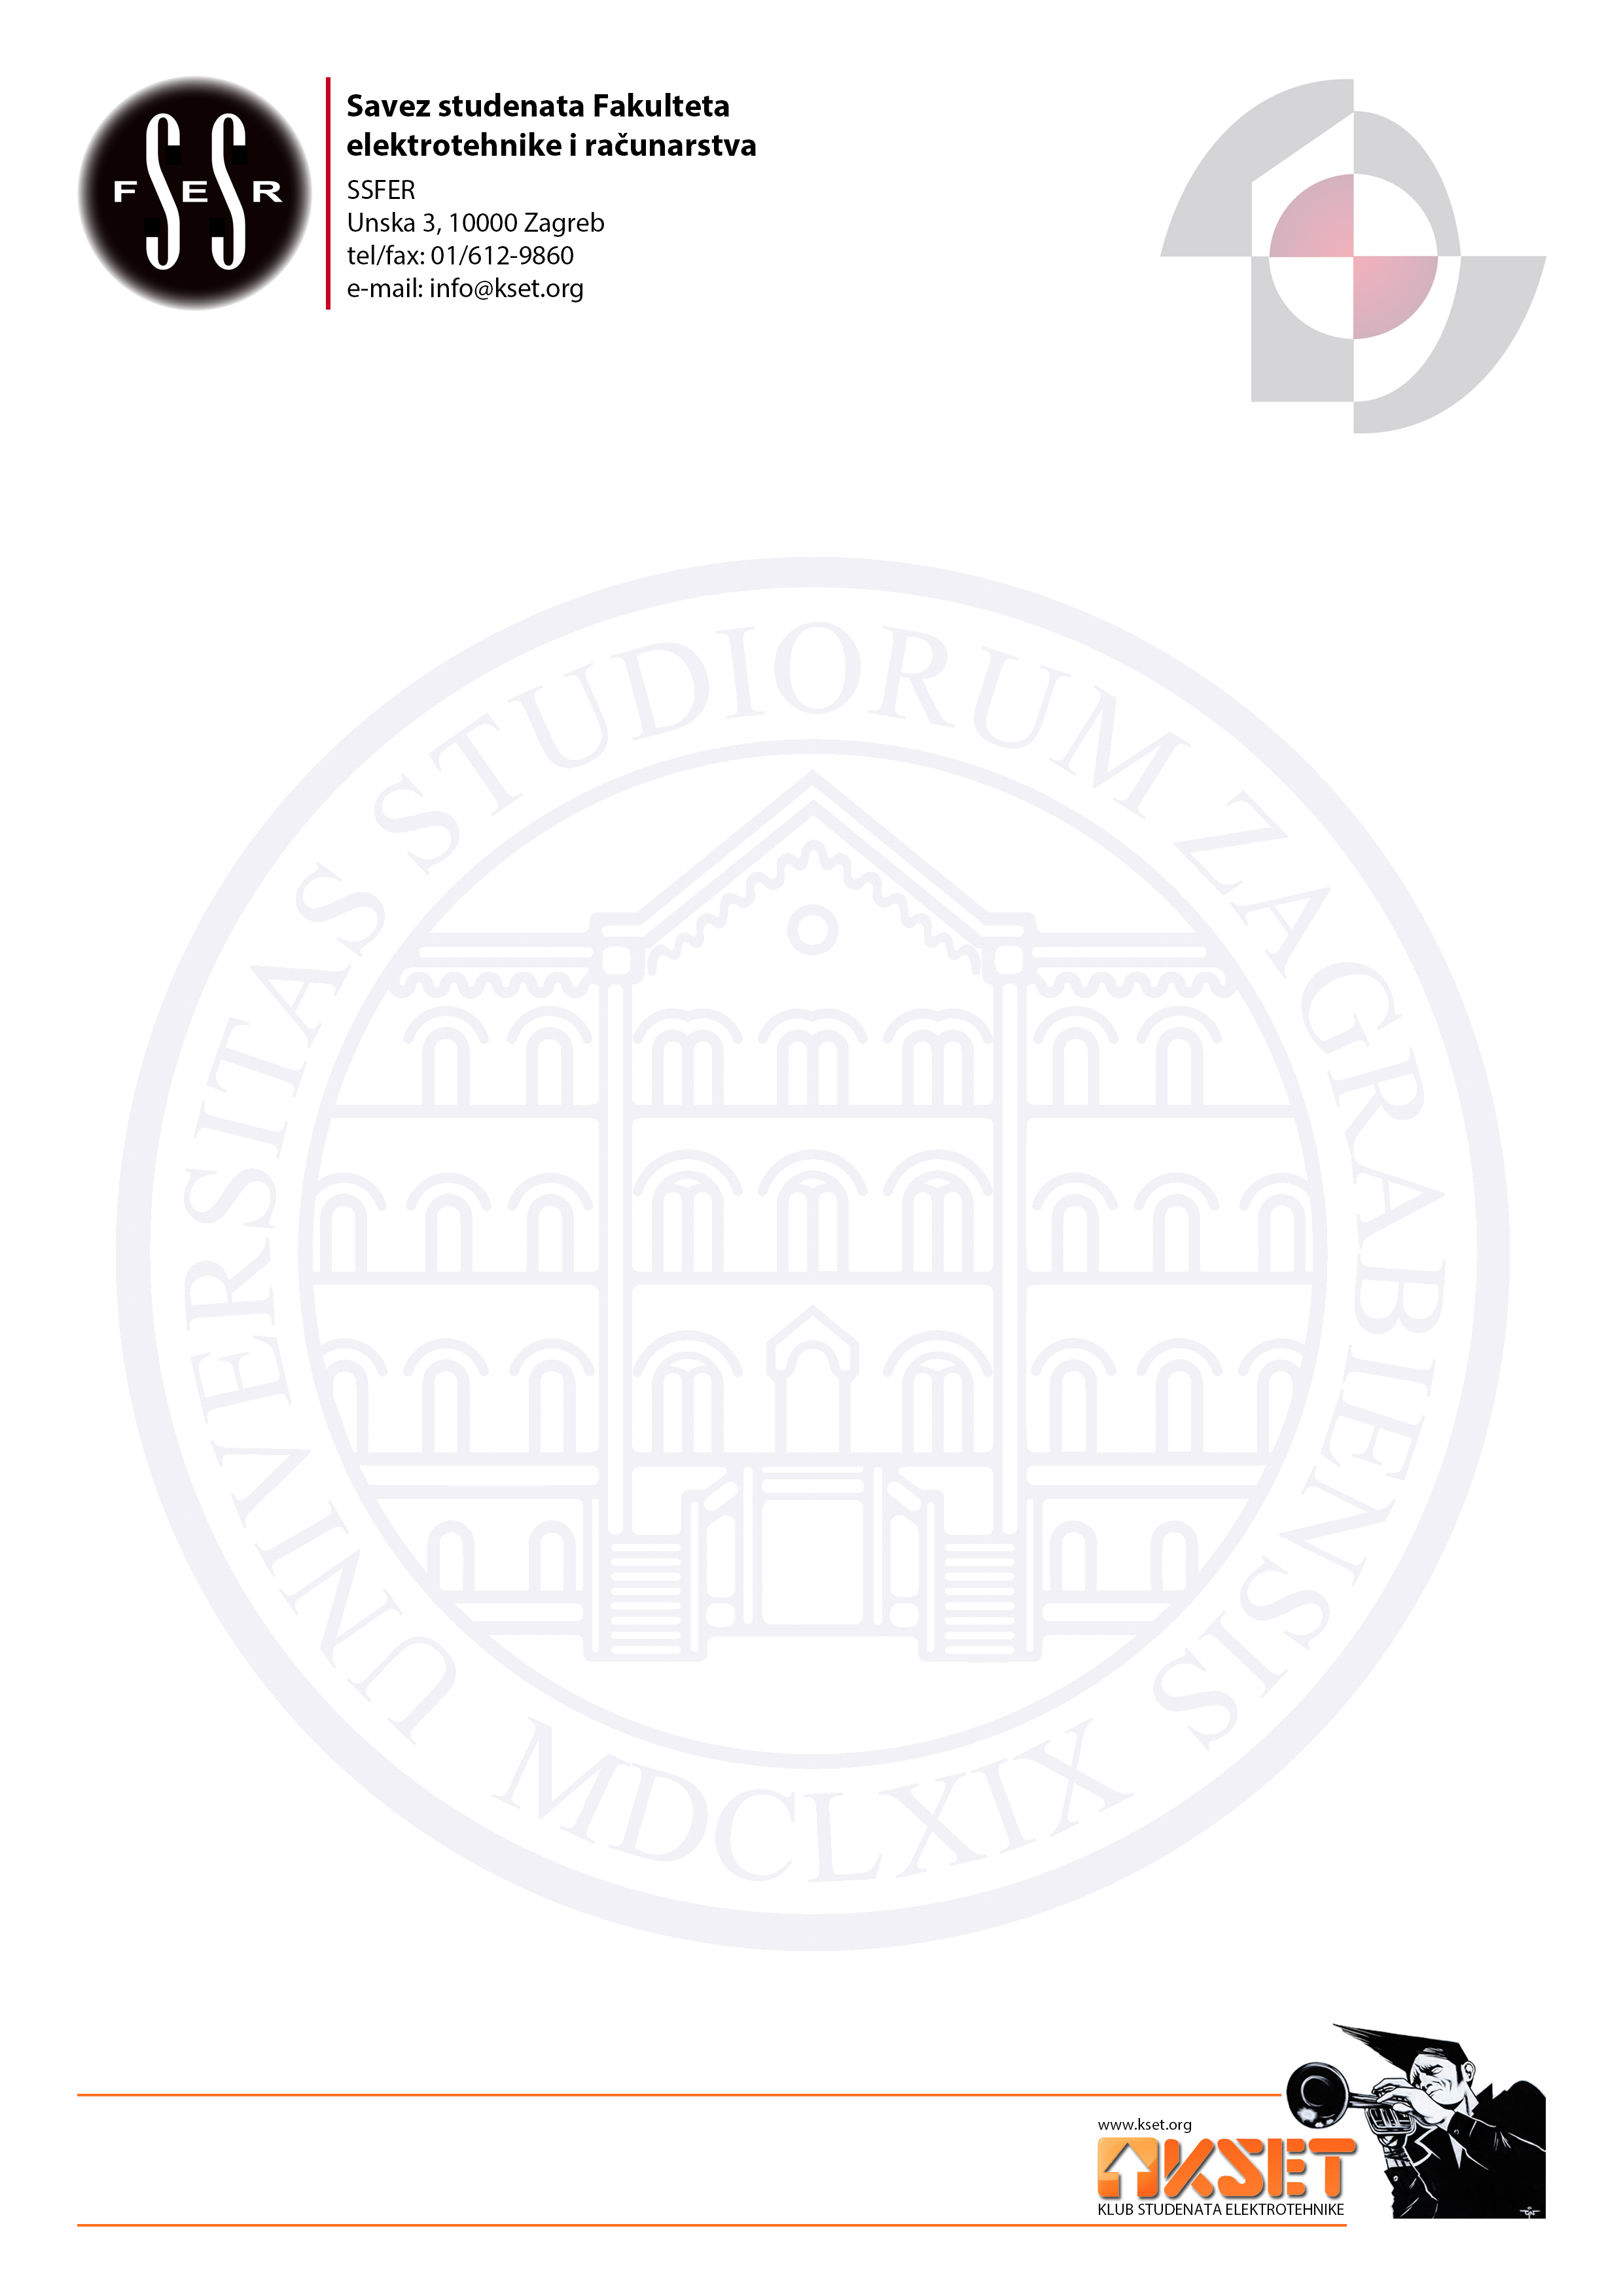
\includegraphics[width=\paperwidth,height=\paperheight]{templateBG}};

\fancyfoot[RE,LO]{\vspace{-7mm} \scriptsize \textbf{SSFER}\\OIB: 14504100702\\Žiro: 2402006-1100582760\\IBAN: HR2324020061100582760 (Erste)}

\section*{O klubu}
\paragraph{} \textbf{Klub studenata elektrotehnike (KSET)} koji djeluje u sklopu Saveza studenata
Fakulteta elektrotehnike i računarstva, jedan je od najstarijih hrvatskih studentskih klubova
koji neprekinuto rade do današnjih dana. Klub okuplja sve zainteresirane studente
Zagrebačkog sveučilišta koji kroz volonterski rad organiziraju i realiziraju kulturne i
edukativne programe (u rasponu od koncerata domaćih i stranih izvođača sve do predstava,
raznih školica i predavanja) te samostalno održavaju čitavu infrastrukturu Kluba. Klub ima
vlastite prostorije među kojima je i dvorana s pozornicom te je cijelu akademsku godinu
otvoren za sve zainteresirane. Ciljana grupa korisnika svih kulturnih i edukativnih klupskih
programa su studenti i mladi. KSET postoji od 1976. godine, a kroz svoje postojanje se dokazao kao
relevantni kulturni čimbenik na nacionalnom nivou i to je ostvario isključivo zbog orijentacije
na studente i mlade.


\paragraph{} \textbf{KSET} je po djelatnostima podijeljen u 9 sekcija koja svaka pokriva jedan aspekt kulturnog života studenata i mladih općenito, a to su: \textbf{Bike sekcija} koja promovira biciklizam te organizira brojne biciklističke izlete i radionice popravljanja bicikla; \textbf{Disco sekcija} koja se brine za glazbenu podlogu svih Klupskih aktivnosti kroz svoje dnevne i noćne DJ programe, organizira škole DJ opreme i miksanja glazbe; \textbf{Dramska sekcija} koja je amaterska kazališna skupina, svake godine izvedu nekoliko predstava vlastite produkcije i organiziraju brojna gostovanja glumačkih skupina; \textbf{Foto sekcija} se bavi fotografijom, organizira školu analogne i digitalne fotografije te u klupskom prostoru organizira brojne gostujuće izložbe fotografija svojih članova i polaznika škole fotografije; \textbf{Glazbena sekcija} se
bavi organizacijom koncerata u prostorijama kluba te ujedno obavlja i sve poslove oko postavljanja i održavanja opreme, organizira školu za tonske operatore; \textbf{Planinarska sekcija} se bavi organizacijom planinarskih izleta za
sve zainteresirane te održava planinarsku školu; \textbf{Računarska sekcija} se bavi održavanjem
interne klupske računarske i mrežne infrastrukture, održavanjem internetskih stranica Kluba,
organizira otvorena predavanja o računarskoj problematici te promiču open source
programe; \textbf{Tehnička sekcija} se bavi
održavanjem fizičkog integriteta kluba (u rasponu od građevinskih, preko vodoinstalaterskih, elektroinstalaterskih pa sve do tesarskih radova) tako i popravcima sve Klupske opreme te u sklopu svog djelovanja imaju brojne škole rukovanja kompliciranijim alatima
kojima pokušavaju mlade naučiti i potaknuti na vlastito rukotvorstvo; \textbf{Video sekcija} se bavi amaterskom produkcijom kratkih igranih i dokumentarnih filmova te organizira javne
projekcije filmskih klasika ili filmova alternativnih sadržaja kojima pokušava obogatiti
kulturnu scenu mladih u Zagrebu.

\newpage
\tikz[remember picture,overlay] \node[opacity=1,inner sep=0pt] at (current page.center){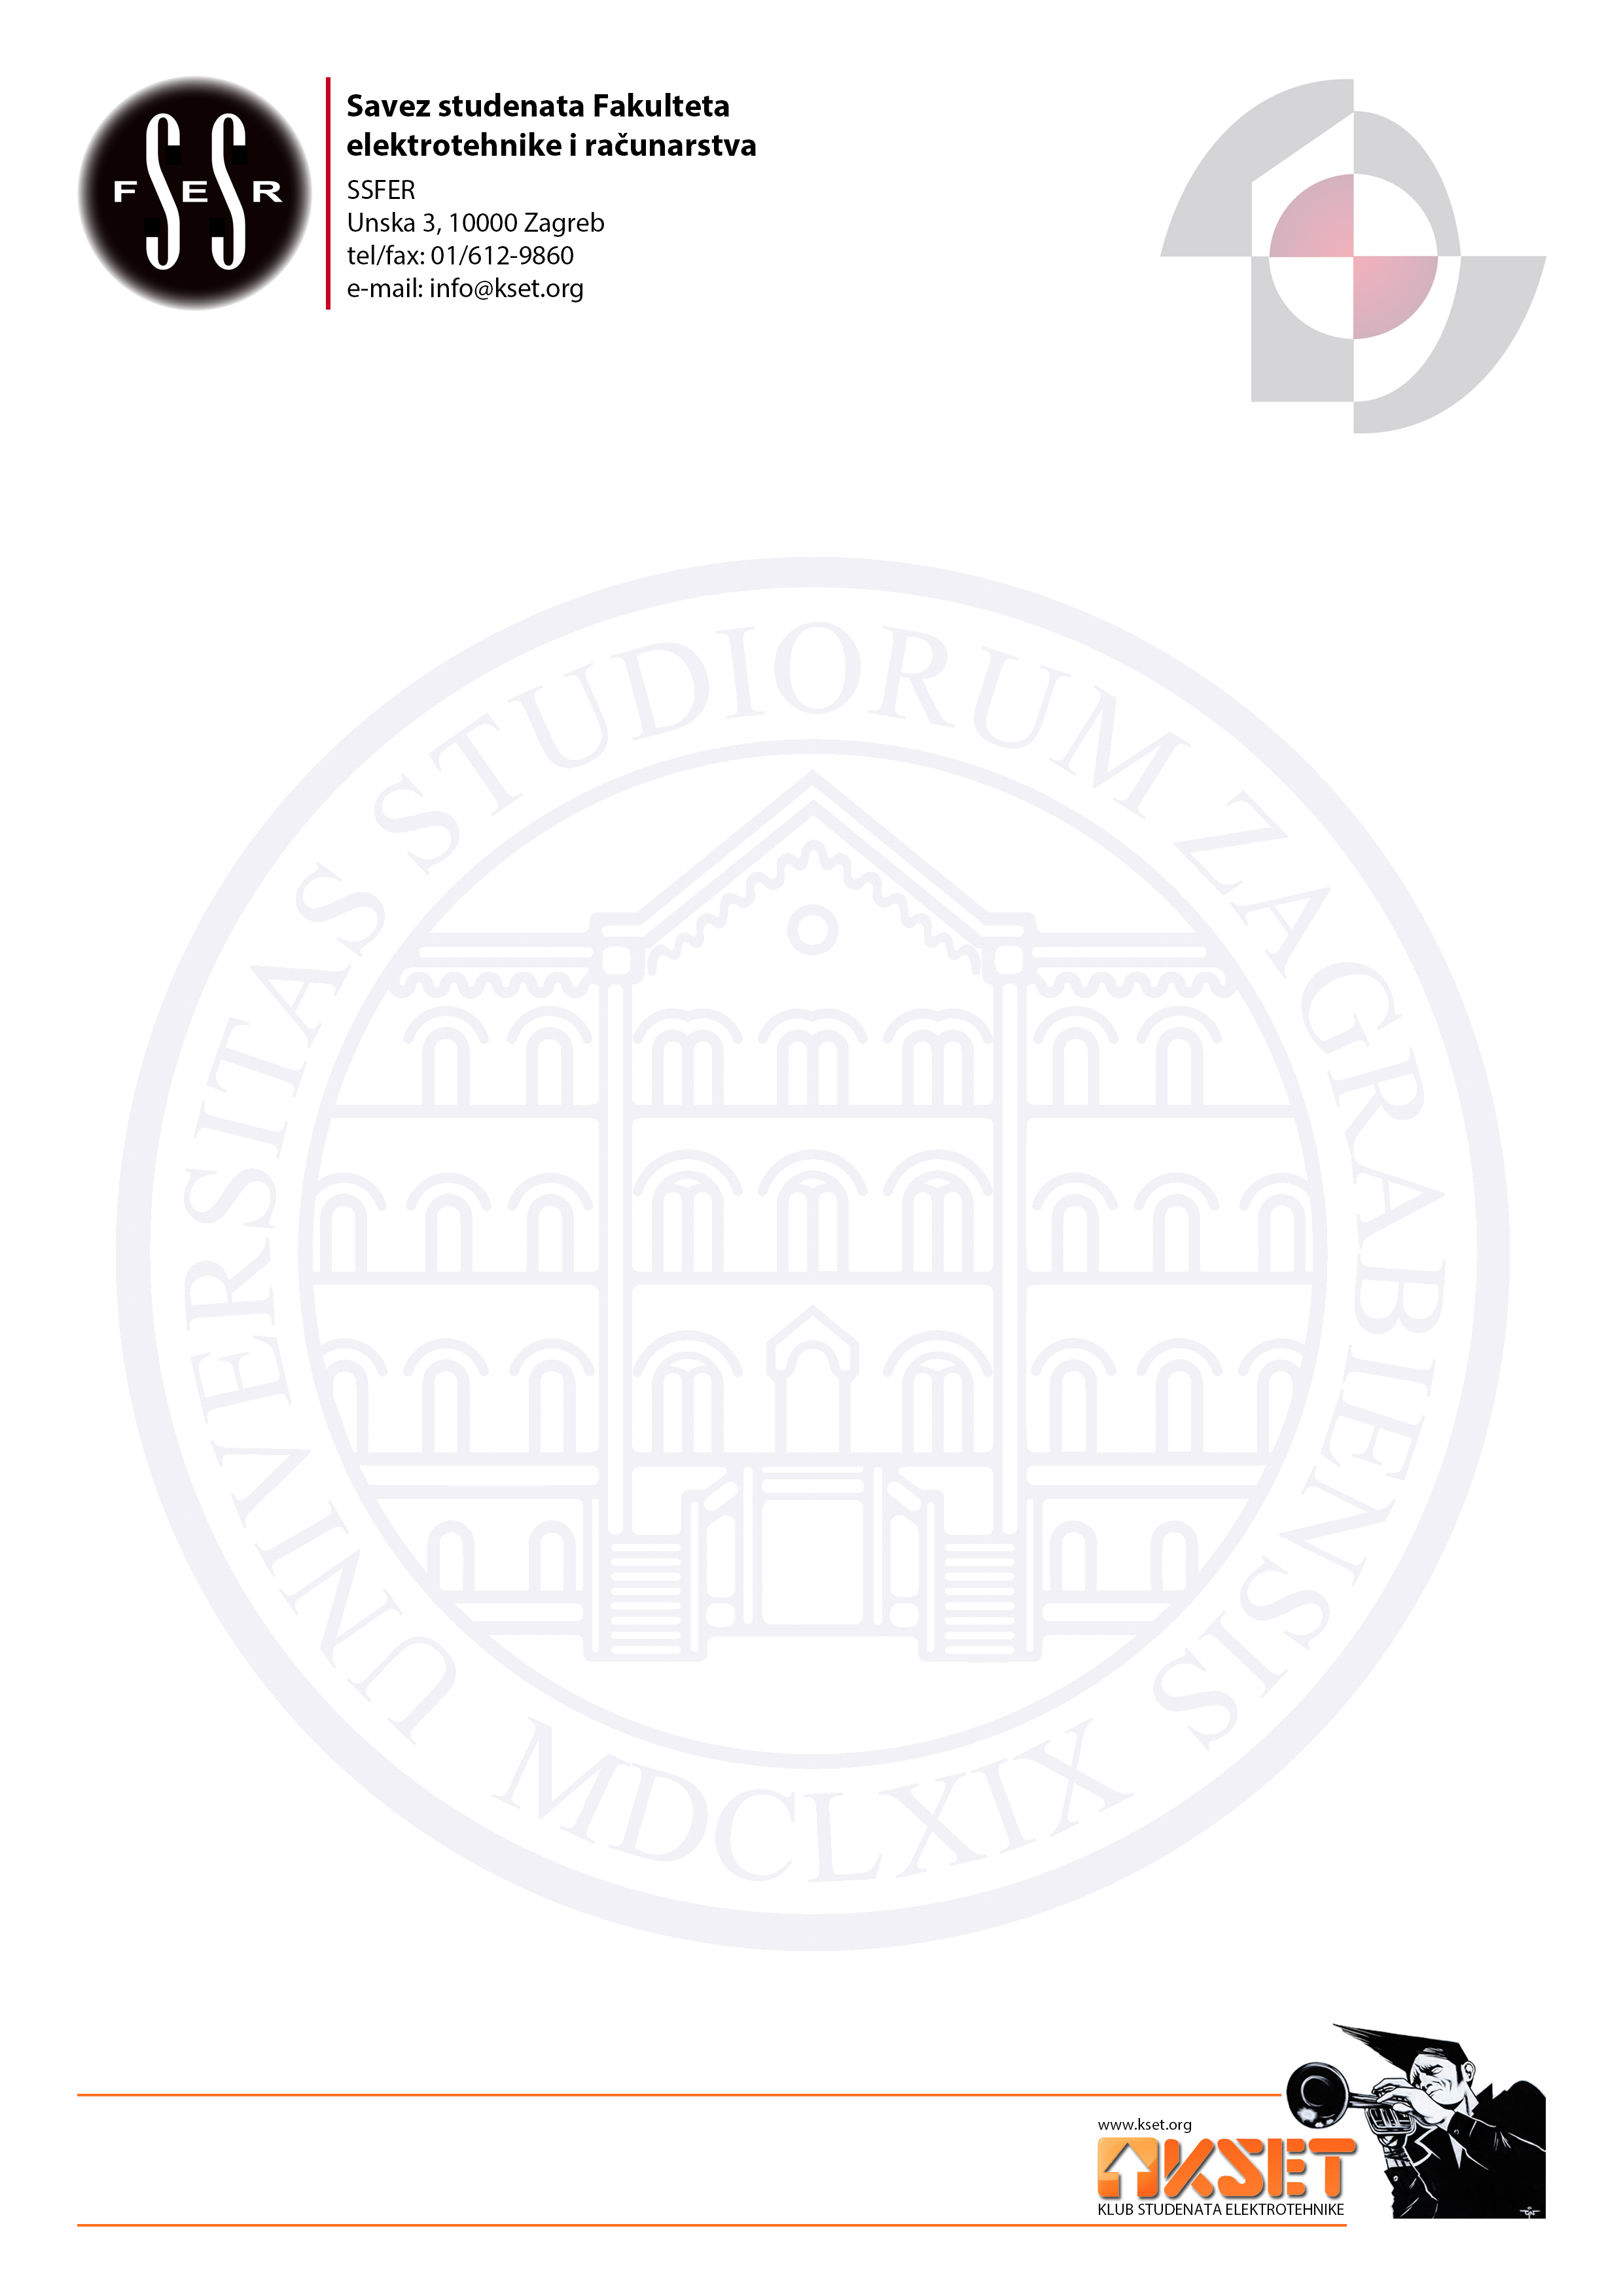
\includegraphics[width=\paperwidth,height=\paperheight]{templateBG}};

\section*{Glazbeno djelovanje}
	
	\paragraph{Brucošijada FER-a}se tradicionalno održava toliko dugo da u KSET-u trenutno ne	postoje članovi koji bi sa sigurnošću znali reći kada je bila prva. Do prije nekoliko	godina brucošijada se održavala na FER-u, a u zadnje 3 godine na alternativnim
	lokacijama (Pauk i SC). Brucošijade FER-a uvijek uključuju 4 podija, svaki sa svojim
	pravcem glazbe kako bi mogli najbolje pokriti različite glazbene ukuse naše publike. 
	
	\begin{wrapfigure}{R}{0.45\textwidth}
		\vspace{-15mm}
		\begin{flushright}
			
\includegraphics[width=0.45\textwidth]{ZARI.png}
		\end{flushright}
		\vspace{-15mm}
	\end{wrapfigure}
	
	\noindent Mnogi danas poznati bendovi svoje su prve velike nastupe održali na Brucošijadi FER-a
	kao Hladno Pivo, TBF, Edo Majka, Toni Cetinski, Darko Rundek, Let 3, Leb i Sol, Urban,
	Gibonni, Stjepan Jimmy Stanić. Ove godine nastavljamo tradiciju pružanja prilike
	mladim, perspektivnim bendovima iz Hrvatske i svijeta kao i nekim već proslavljenim
	bendovima.

	\vspace{1cm}
	
	\paragraph{Čuješ?!}je program kojim želimo dati priliku nastupa i promocije manje afirmiranim, ali izrazito kvalitetnim bendova iz cijele Hrvatske koji zbog okupiranosti medija mainstream glazbom nezasluženo ne dobivaju dovoljno medijske pažnje, pa je samim tim i interes publike za njima manji. Sukladno tome zatvaraju im se i mnoga mjesta za nastup koja se vode isključivo financijskom dobiti. Program stavlja naglasak na kvalitetu izvođača s ciljem da u konačnici ostvari pozitivnu nulu, a da s druge strane izvođači dobiju minimalno potrebne uvjete da bi mogli dići na nastup u vidu smještaja, cateringa i putnih troškova.
	
	\vspace{1cm}
	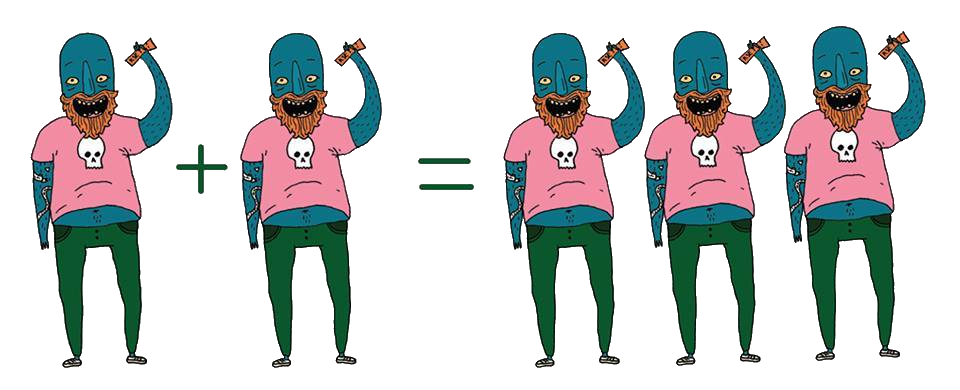
\includegraphics[scale=0.5]{cujes.png}
	
	\newpage
	\tikz[remember picture,overlay] \node[opacity=1,inner sep=0pt] at (current page.center){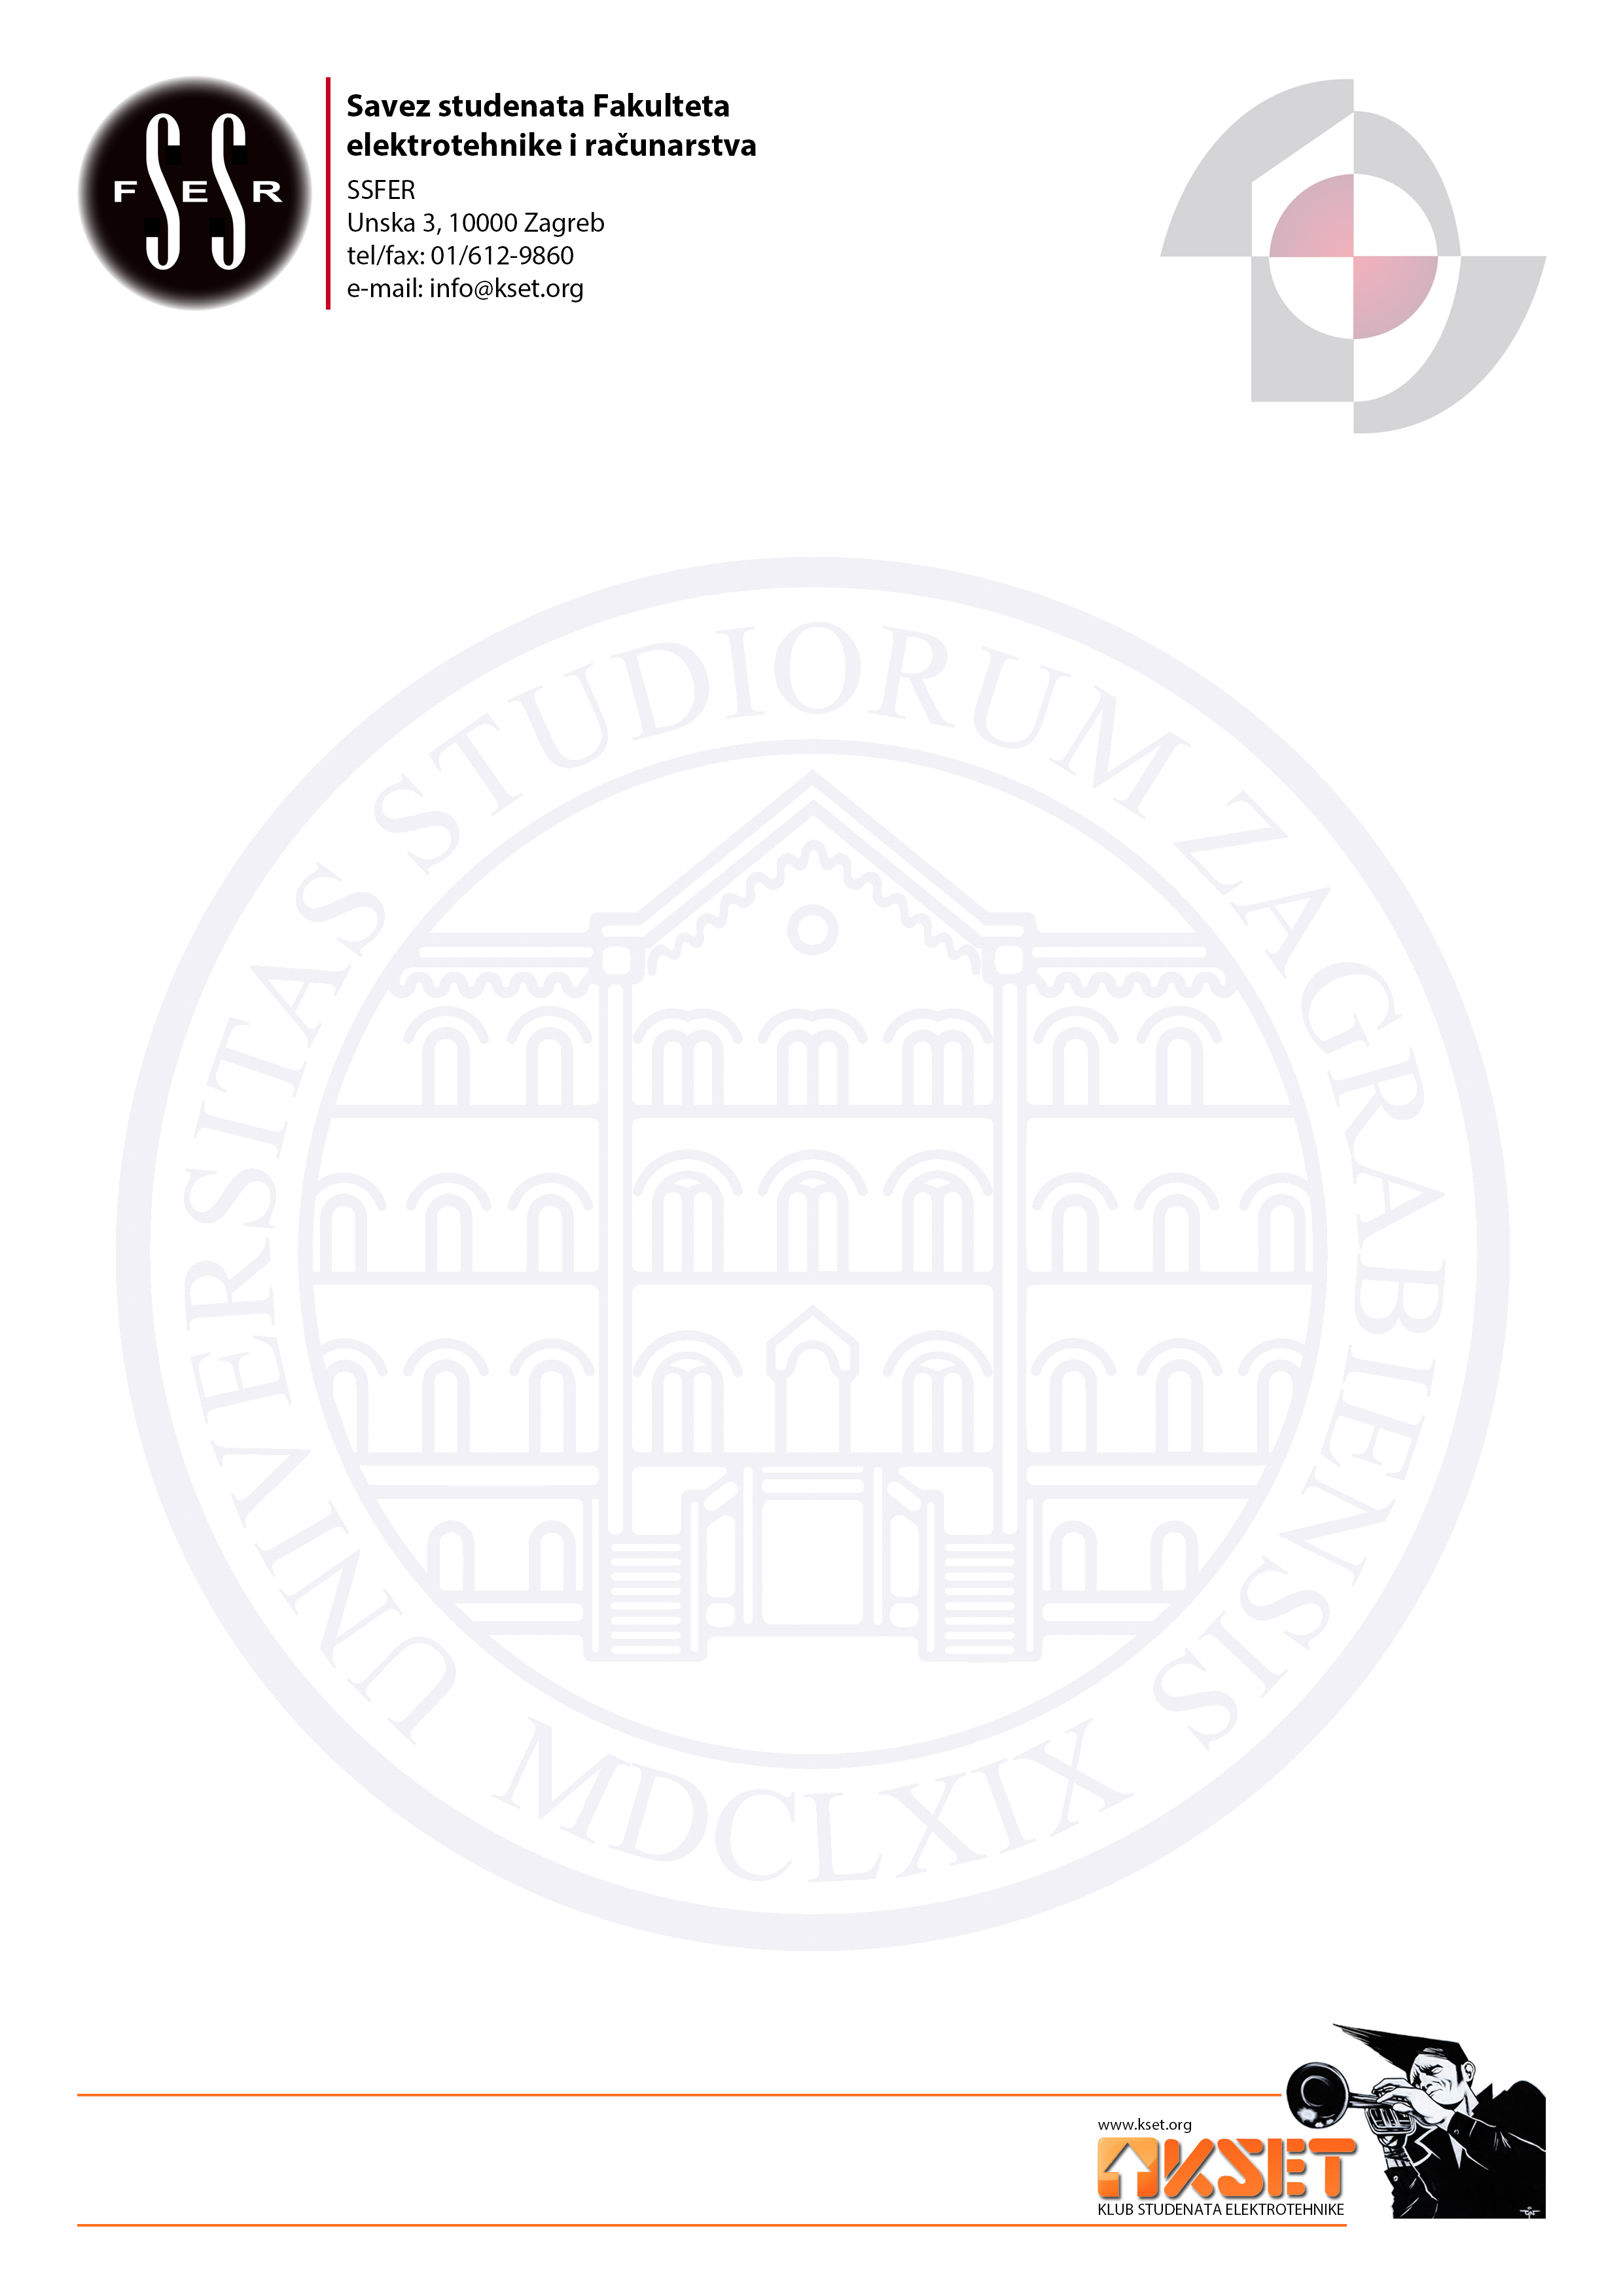
\includegraphics[width=\paperwidth,height=\paperheight]{templateBG}};	
	
	\paragraph{Zavod za eksperimentalni zvuk}je program posvećenoj avangardnoj glazbi s naglaskom na eksperimentalni jazz. Jazz je jedna od osnovica suvremene glazbene umjetnosti i njegov utjecaj je nemjerljiv, preljevajući se u sve suvremene glazbene pravce. Kroz godine jazz je razvio bogatstvo podžanrova i kao takav ostavio utjecaj na kulturni pejzaž svakog europskog kulturnog središta. KSET je oduvijek bio mjesto koje je promovirao jazz kao standard urbane kulture, a poslužio je i kao inkubator u kojem su se razvili značajni kulturni festivali. Primarni cilj je stvoriti studentsku publiku ove glazbe koja se nalazi van formata radio postaja, ali i van formata zabavne i kulturne ponude u Zagrebu. 
			
	\begin{figure}[h!]
		\centering
		\vspace{5mm}
		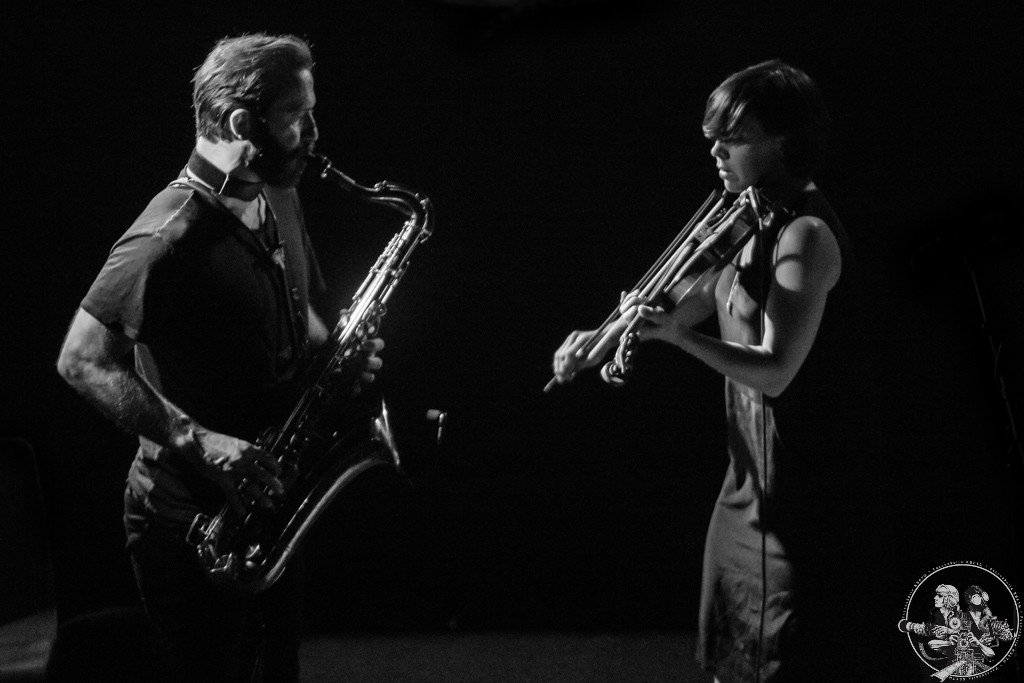
\includegraphics[scale=0.25]{zez.jpg}	
	\end{figure}
	
\newpage
\tikz[remember picture,overlay] \node[opacity=1,inner sep=0pt] at (current page.center){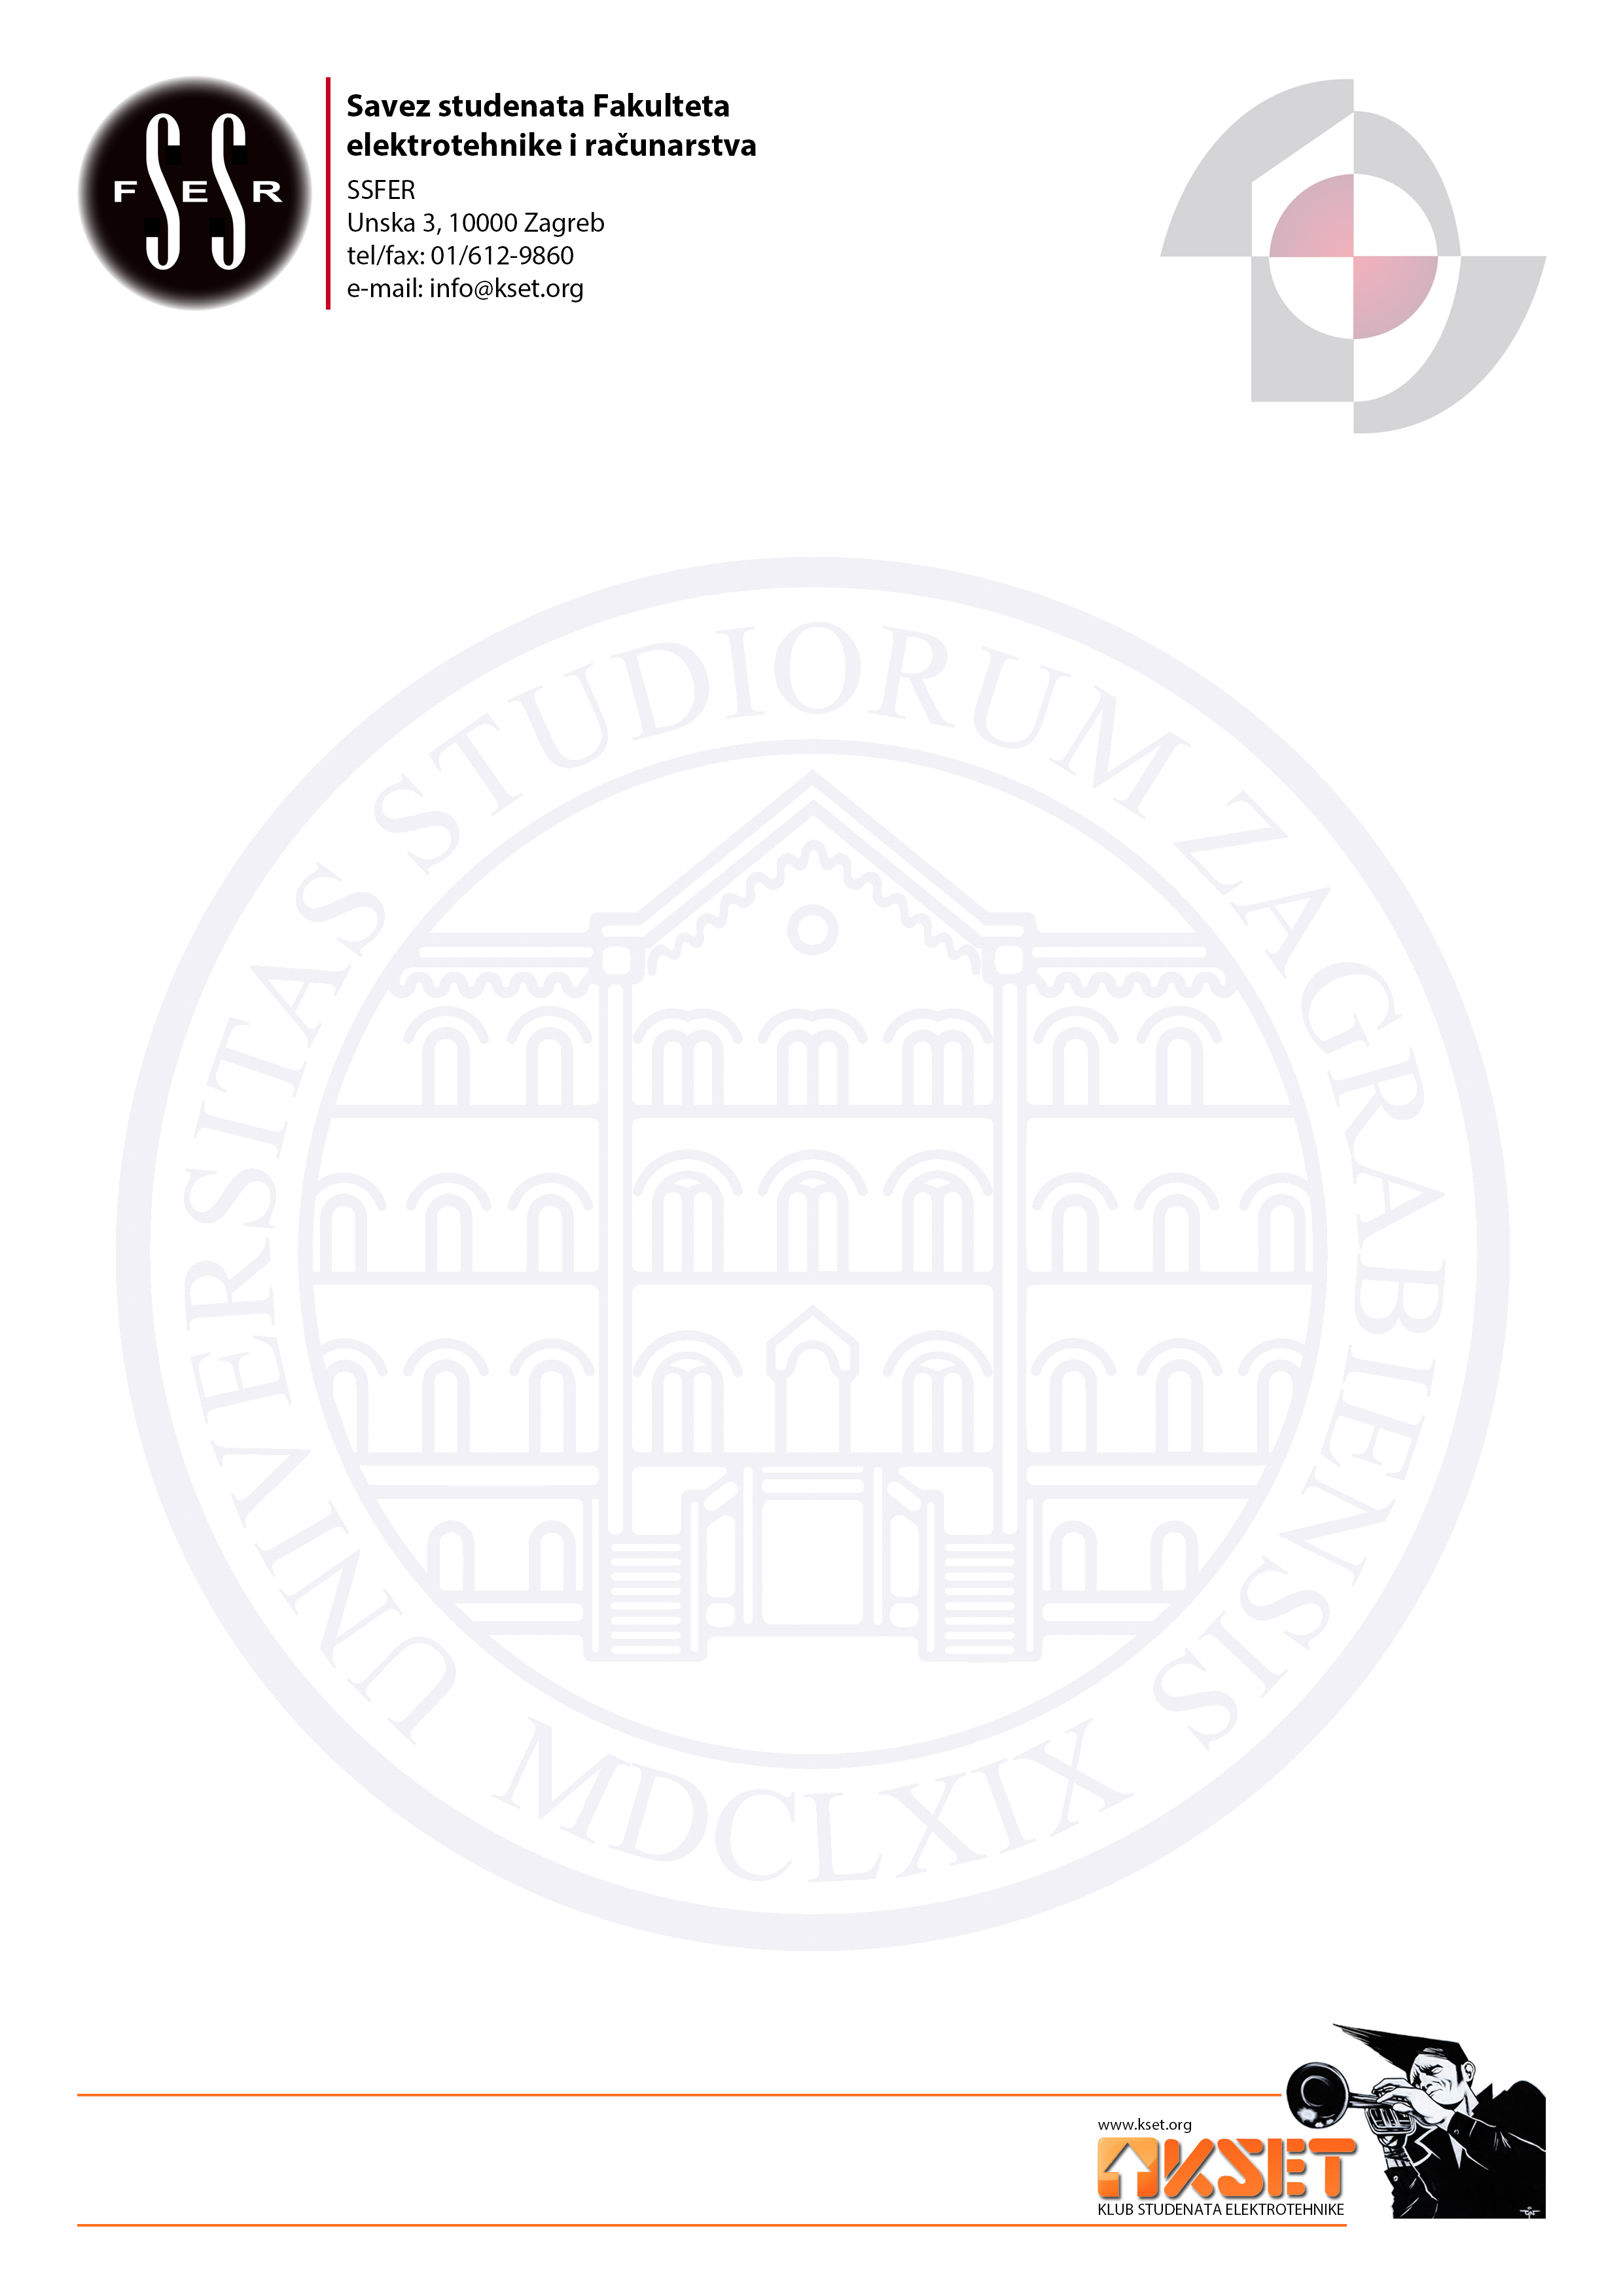
\includegraphics[width=\paperwidth,height=\paperheight]{templateBG}};

\section*{Kulturno djelovanje}

	\paragraph{Srijednjak}je najraznolikiji večernji program u KSET-u. Obuhvaća mnogo formi i tematika: od viteških turnira, preko slušaonica, do različitih natjecanja (videoigre, pjevanje, mimika i drugo), a zajedničko im je to da se događa srijedom.

	\paragraph{Stiholoporter}je novi program Dramske sekcije KSET-a koji obuhvaća nekoliko aspekata studentske literarne kulture. Kao centralni događaji programa tu su večeri poezije, večeri kada se u mirnoj  nedjeljnoj atmosferi Kluba čita odabrana poezija. Na repertoaru su svjetski klasici kao i moderna poezija i proza, te autorska djela samih članova kao i studenata van udruge. Putem naše web stranice i društvenih mreža na mjesečnoj bazi raspisujemo natječaj za prijavu studentskih uradaka. Nakon selekcije, autori nam ustupaju svoje uratke koje potom izvodimo, ili ih izvode sami autori.
	
	\begin{figure}[h!]
		\centering
		\vspace{5mm}
		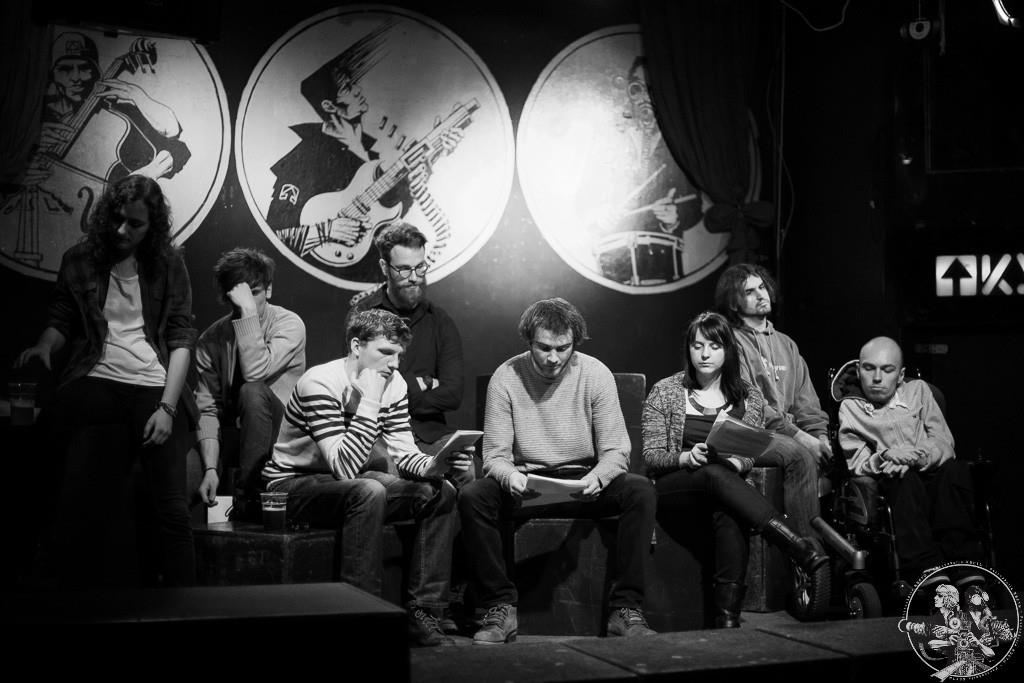
\includegraphics[scale=0.3]{stiholoporter.jpg}	
	\end{figure}
	
\newpage
\tikz[remember picture,overlay] \node[opacity=1,inner sep=0pt] at (current page.center){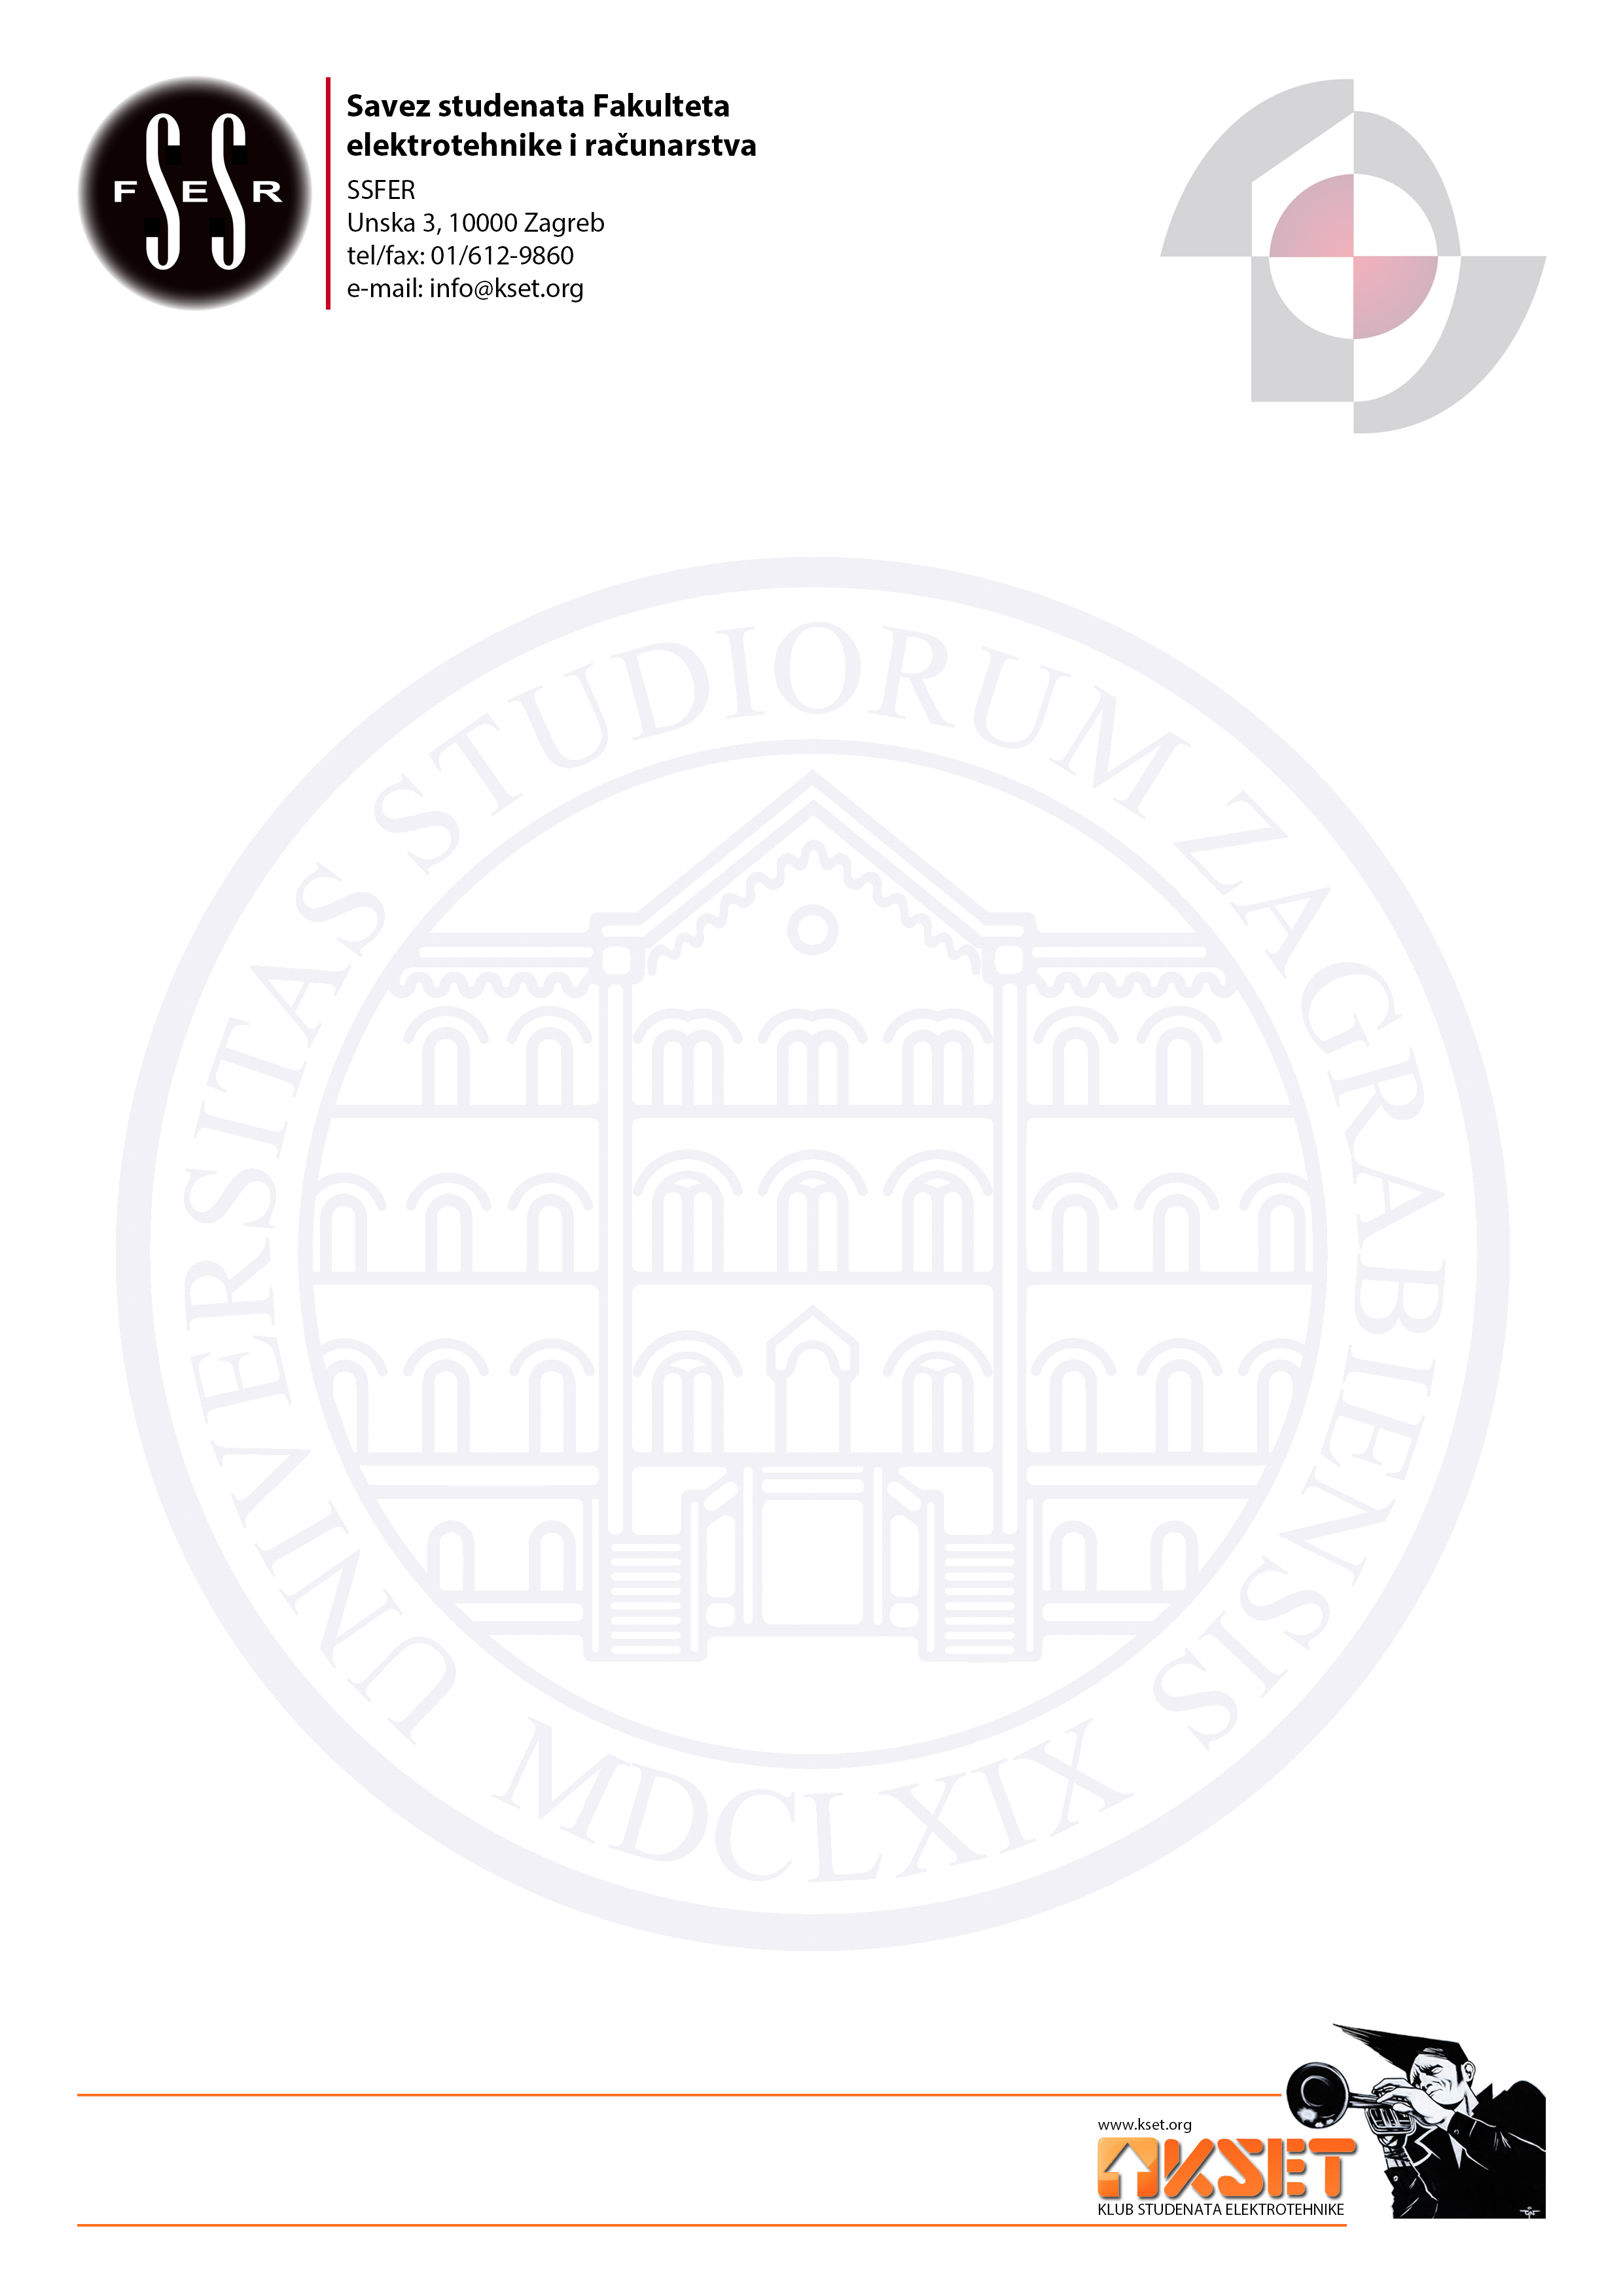
\includegraphics[width=\paperwidth,height=\paperheight]{templateBG}};
	
	\paragraph{play@kset}se svodi na produkciju vlastitih predstava (nekoliko u sezoni) te organiziranje gostovanja predstava vanjske produkcije (studentskih glumačkih skupina, amaterskih družina, studenata Akademije dramskih umjetnosti i renomiranih glumaca) jednom mjesečno u KSET-u. 
	
	\begin{figure}[h!]
		\centering
		\vspace{5mm}
		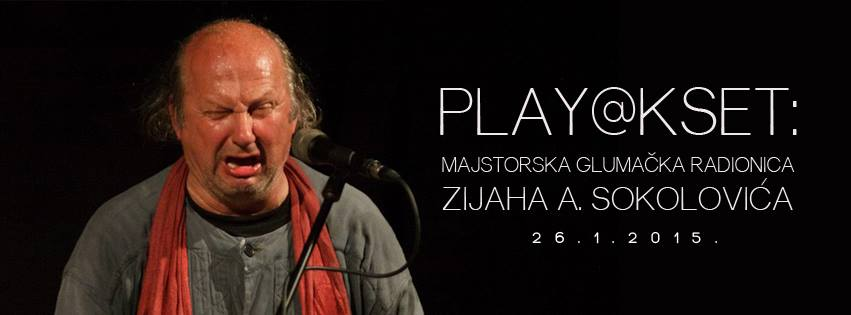
\includegraphics[scale=0.45]{play.jpg}	
	\end{figure}
	
	\paragraph{Foto izložbe}su izložbe gdje Foto sekcija ima potrebu izložiti produkt svoga rada. Iz tog se razloga održavaju izložbe fotografija. KSET je omogućio prostor sekciji za izlaganje radova na neograničeno vrijeme, tako da su jedina zapreka stalnom održavanju izložbi financije.
	
	\paragraph{Fotoputokazi}su program koji se sastoji od jednodnevnog putovanja na odabranu lokaciju, organiziranog grupnog fotografiranja pod vodstvom starijih članova fotosekcije, zajedničkog ručka i povratka kući.               Lokacije se odabiru po kriteriju kulturoloških zanimljivosti i motiva te po kriteriju pogodnosti za razvijanje fotografskih vještina i korištenje različitih fotografskih tehnika i opreme.

\newpage
\tikz[remember picture,overlay] \node[opacity=1,inner sep=0pt] at (current page.center){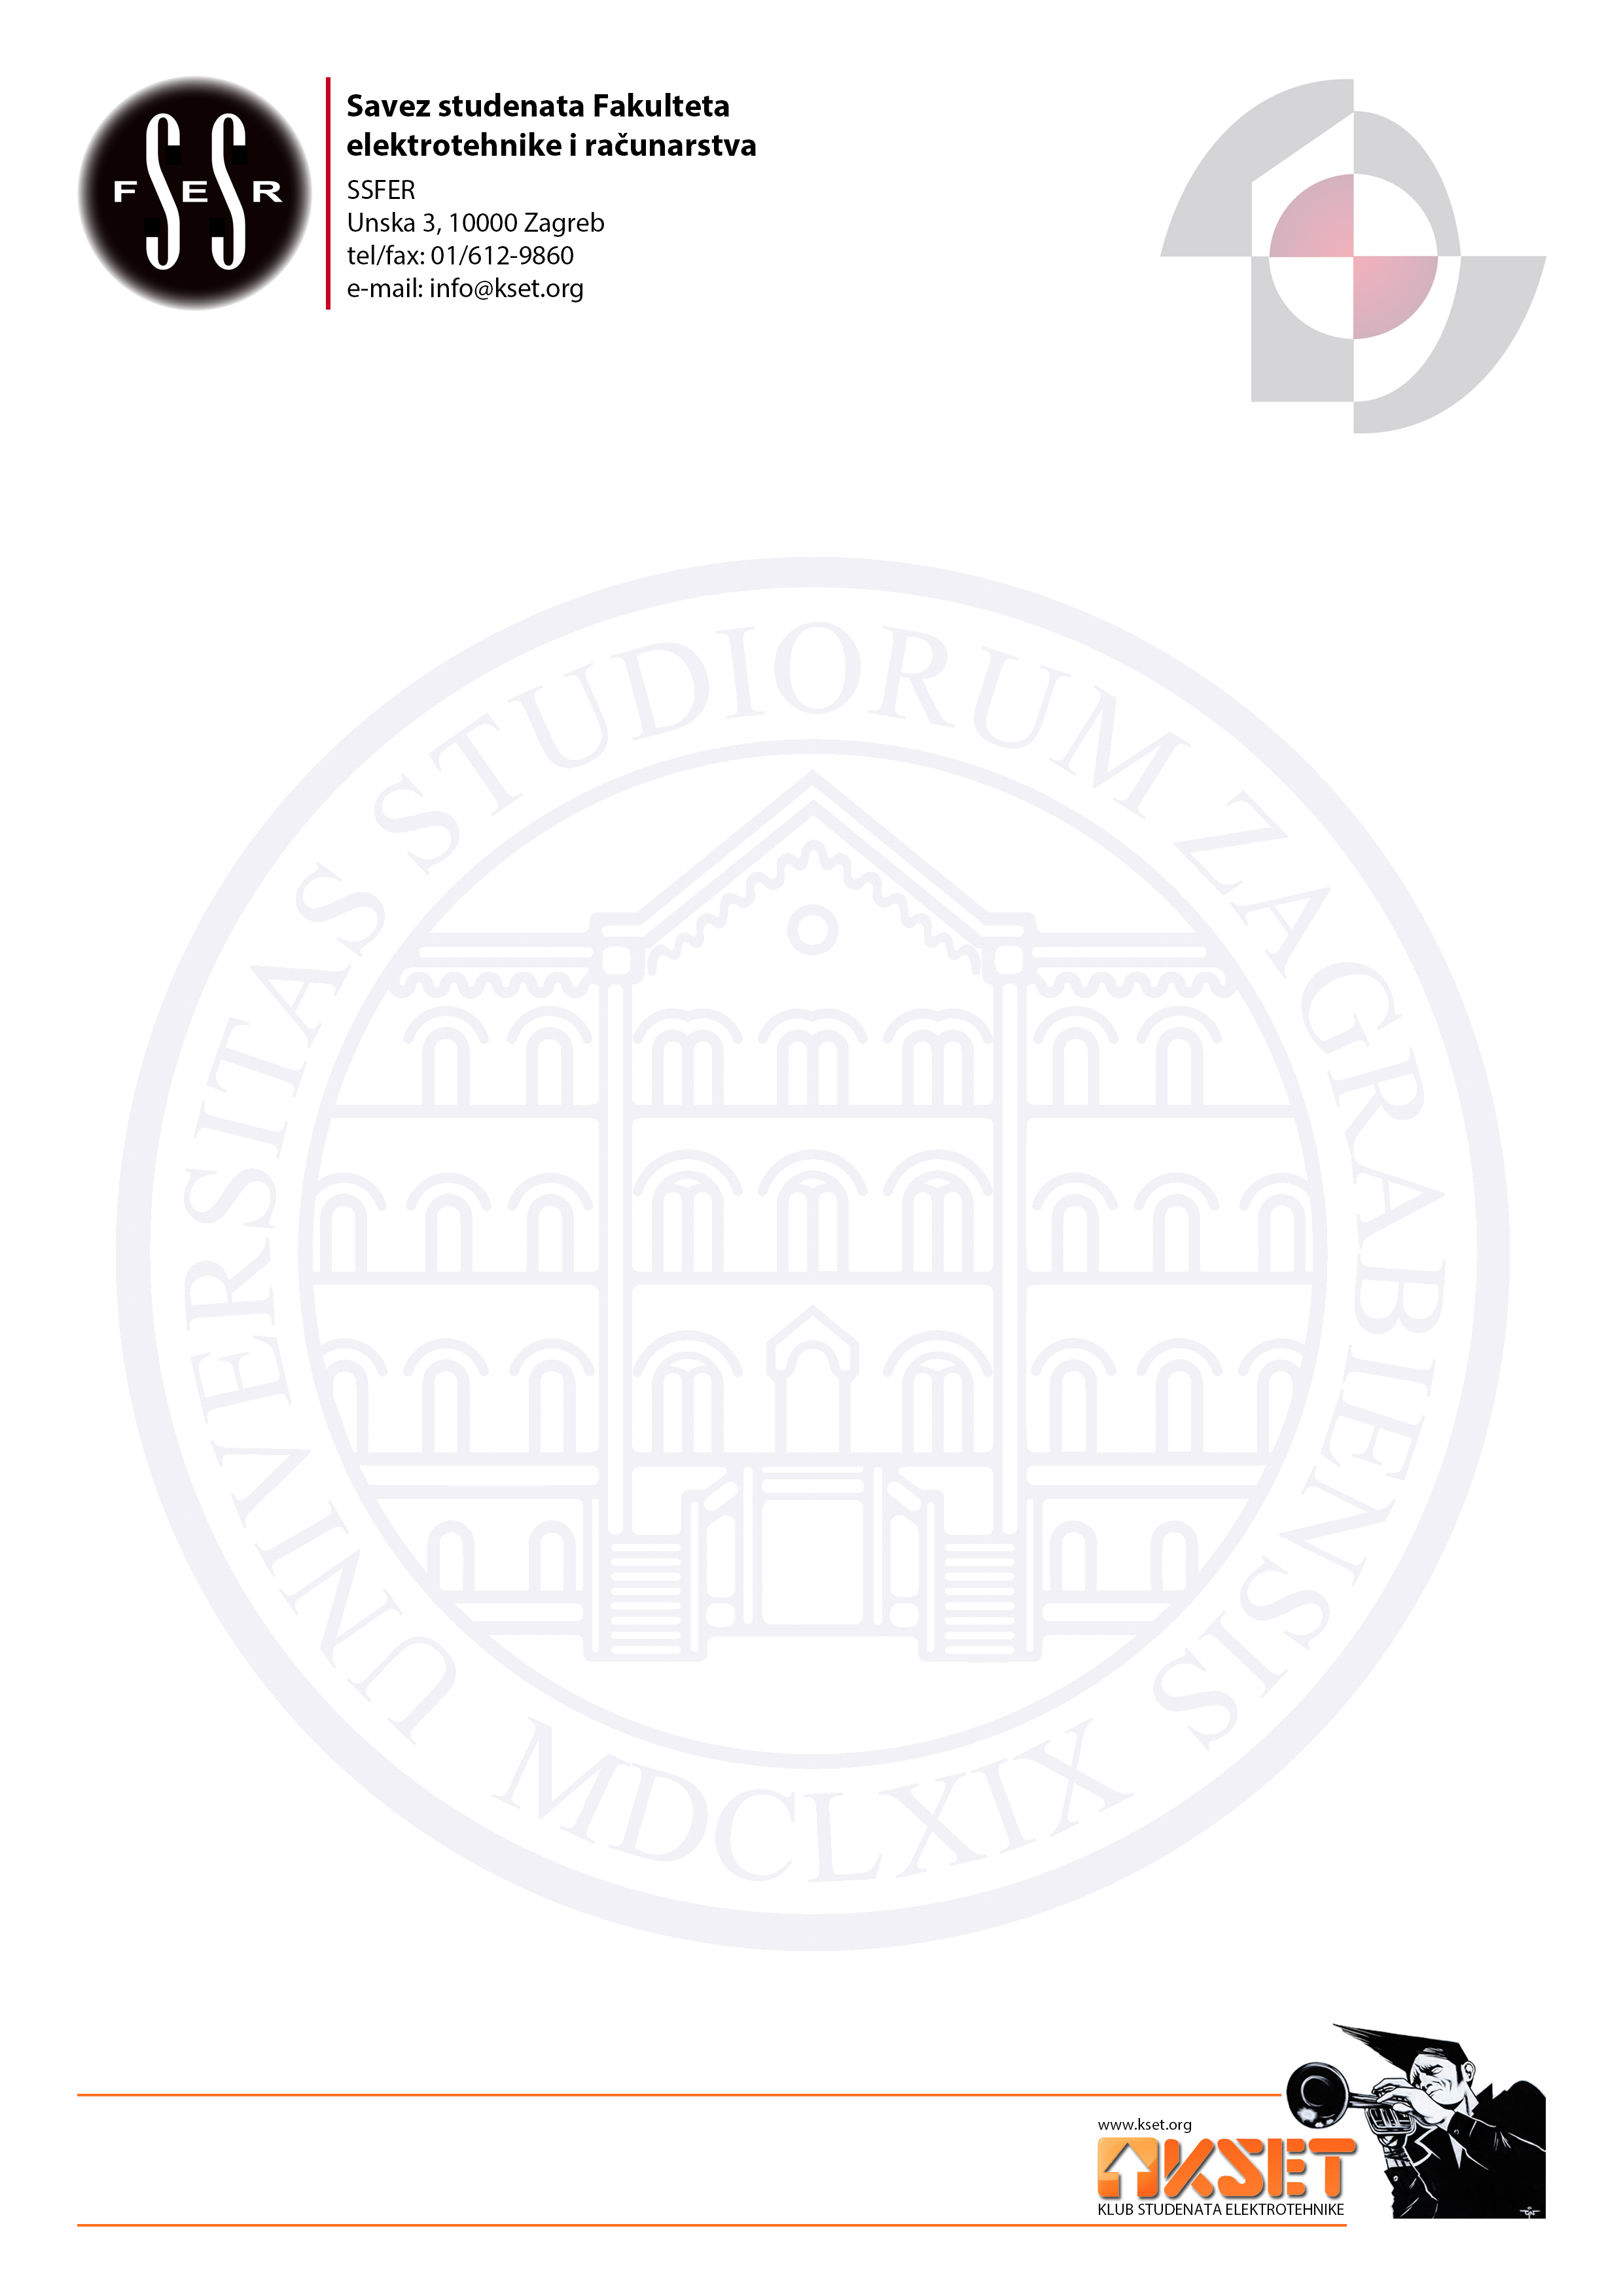
\includegraphics[width=\paperwidth,height=\paperheight]{templateBG}};
	
	\paragraph{Elektrolaninarski Rally}je događaj sportsko-zabavnog karaktera koji okuplja studente, asistente i profesore kroz cjelodnevno planinarsko iskustvo začinjeno igrama i zagonetkama. Rally ima tradiciju održavanja koja se proteže od 1976. g. uz prekid održavanja tijekom Domovinskog rata. Rally je spoj ugodnog druženja, ne prenapornog planinarenja na atraktivnim lokacijama, orijentacije u prirodi, šaljivih i poučnih pitanja iz opće kulture, elektrotehnike, matematike, ekologije, biologije i sličnih znanosti, igara “bez granica” te večernje zabave s objavom rezultata i dodjelom diploma i nagrada najuspješnijim ekipama.
	
	\begin{figure}[h!]
		\centering
		\vspace{5mm}
		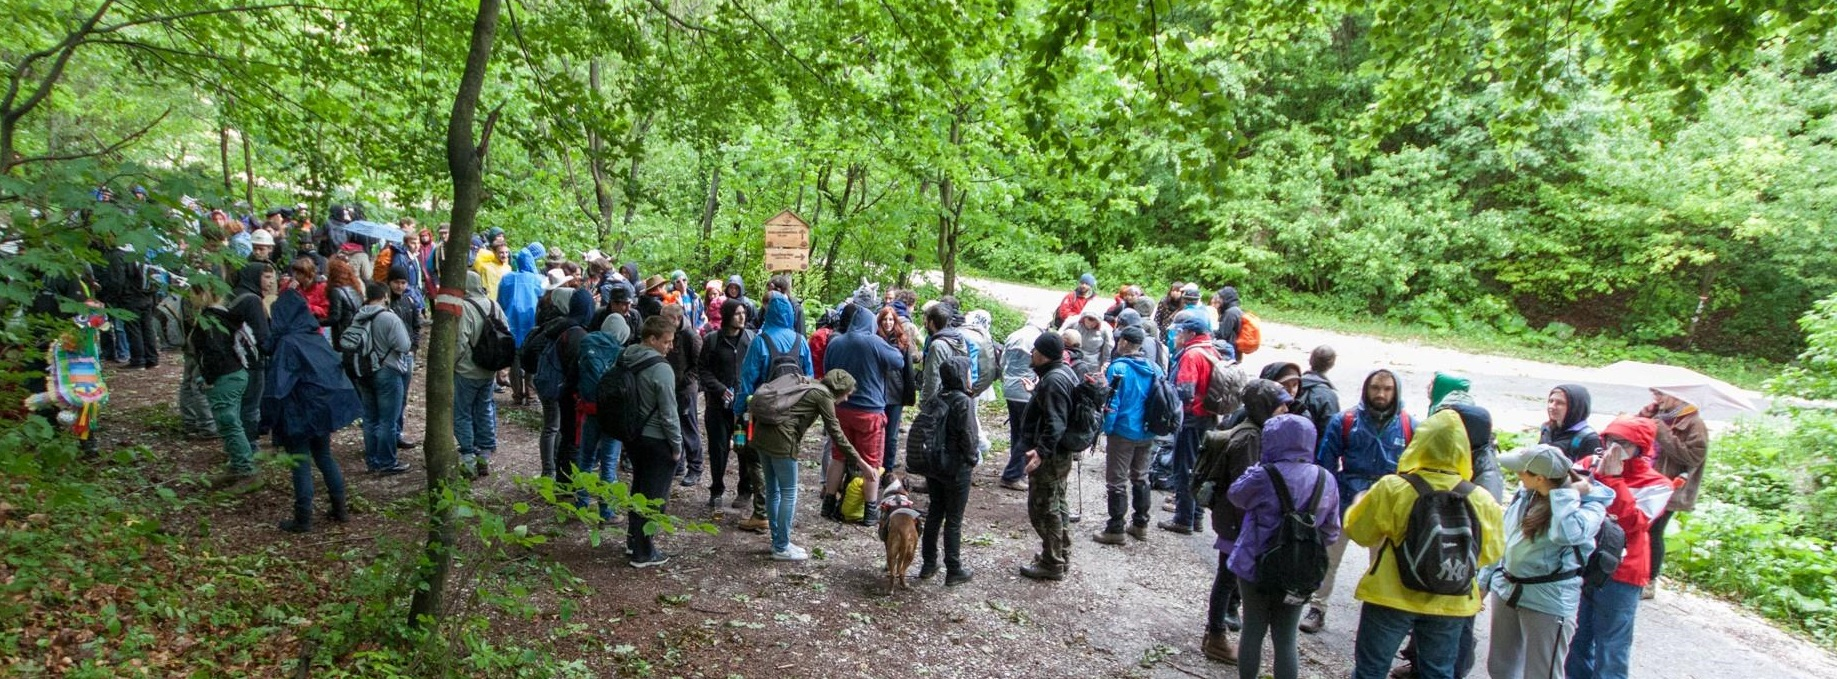
\includegraphics[scale=0.28]{rally1.jpg}	
	\end{figure}
	
	\paragraph{Projekcije filmova}su filmske projekcije sa svrhom informiranja i edukacije svih koji pokažu zanimanje za ovu granu umjetnosti, a posebno studenata. Ovaj program provodi se kroz redovne filmske večeri na kojima se prikazuju animirani, dokumentarni i igrani filmovi, od kojih su mnogi iz vlastite produkcije. U sklopu filmskih večeri događa se i Dvoboj filmova, dvostruka projekcija jednog alternativnog i jednog popularnog filma sa sličnom temom, s ciljem usporedbe dva različita pogleda na istu problematiku.
	
\newpage
\tikz[remember picture,overlay] \node[opacity=1,inner sep=0pt] at (current page.center){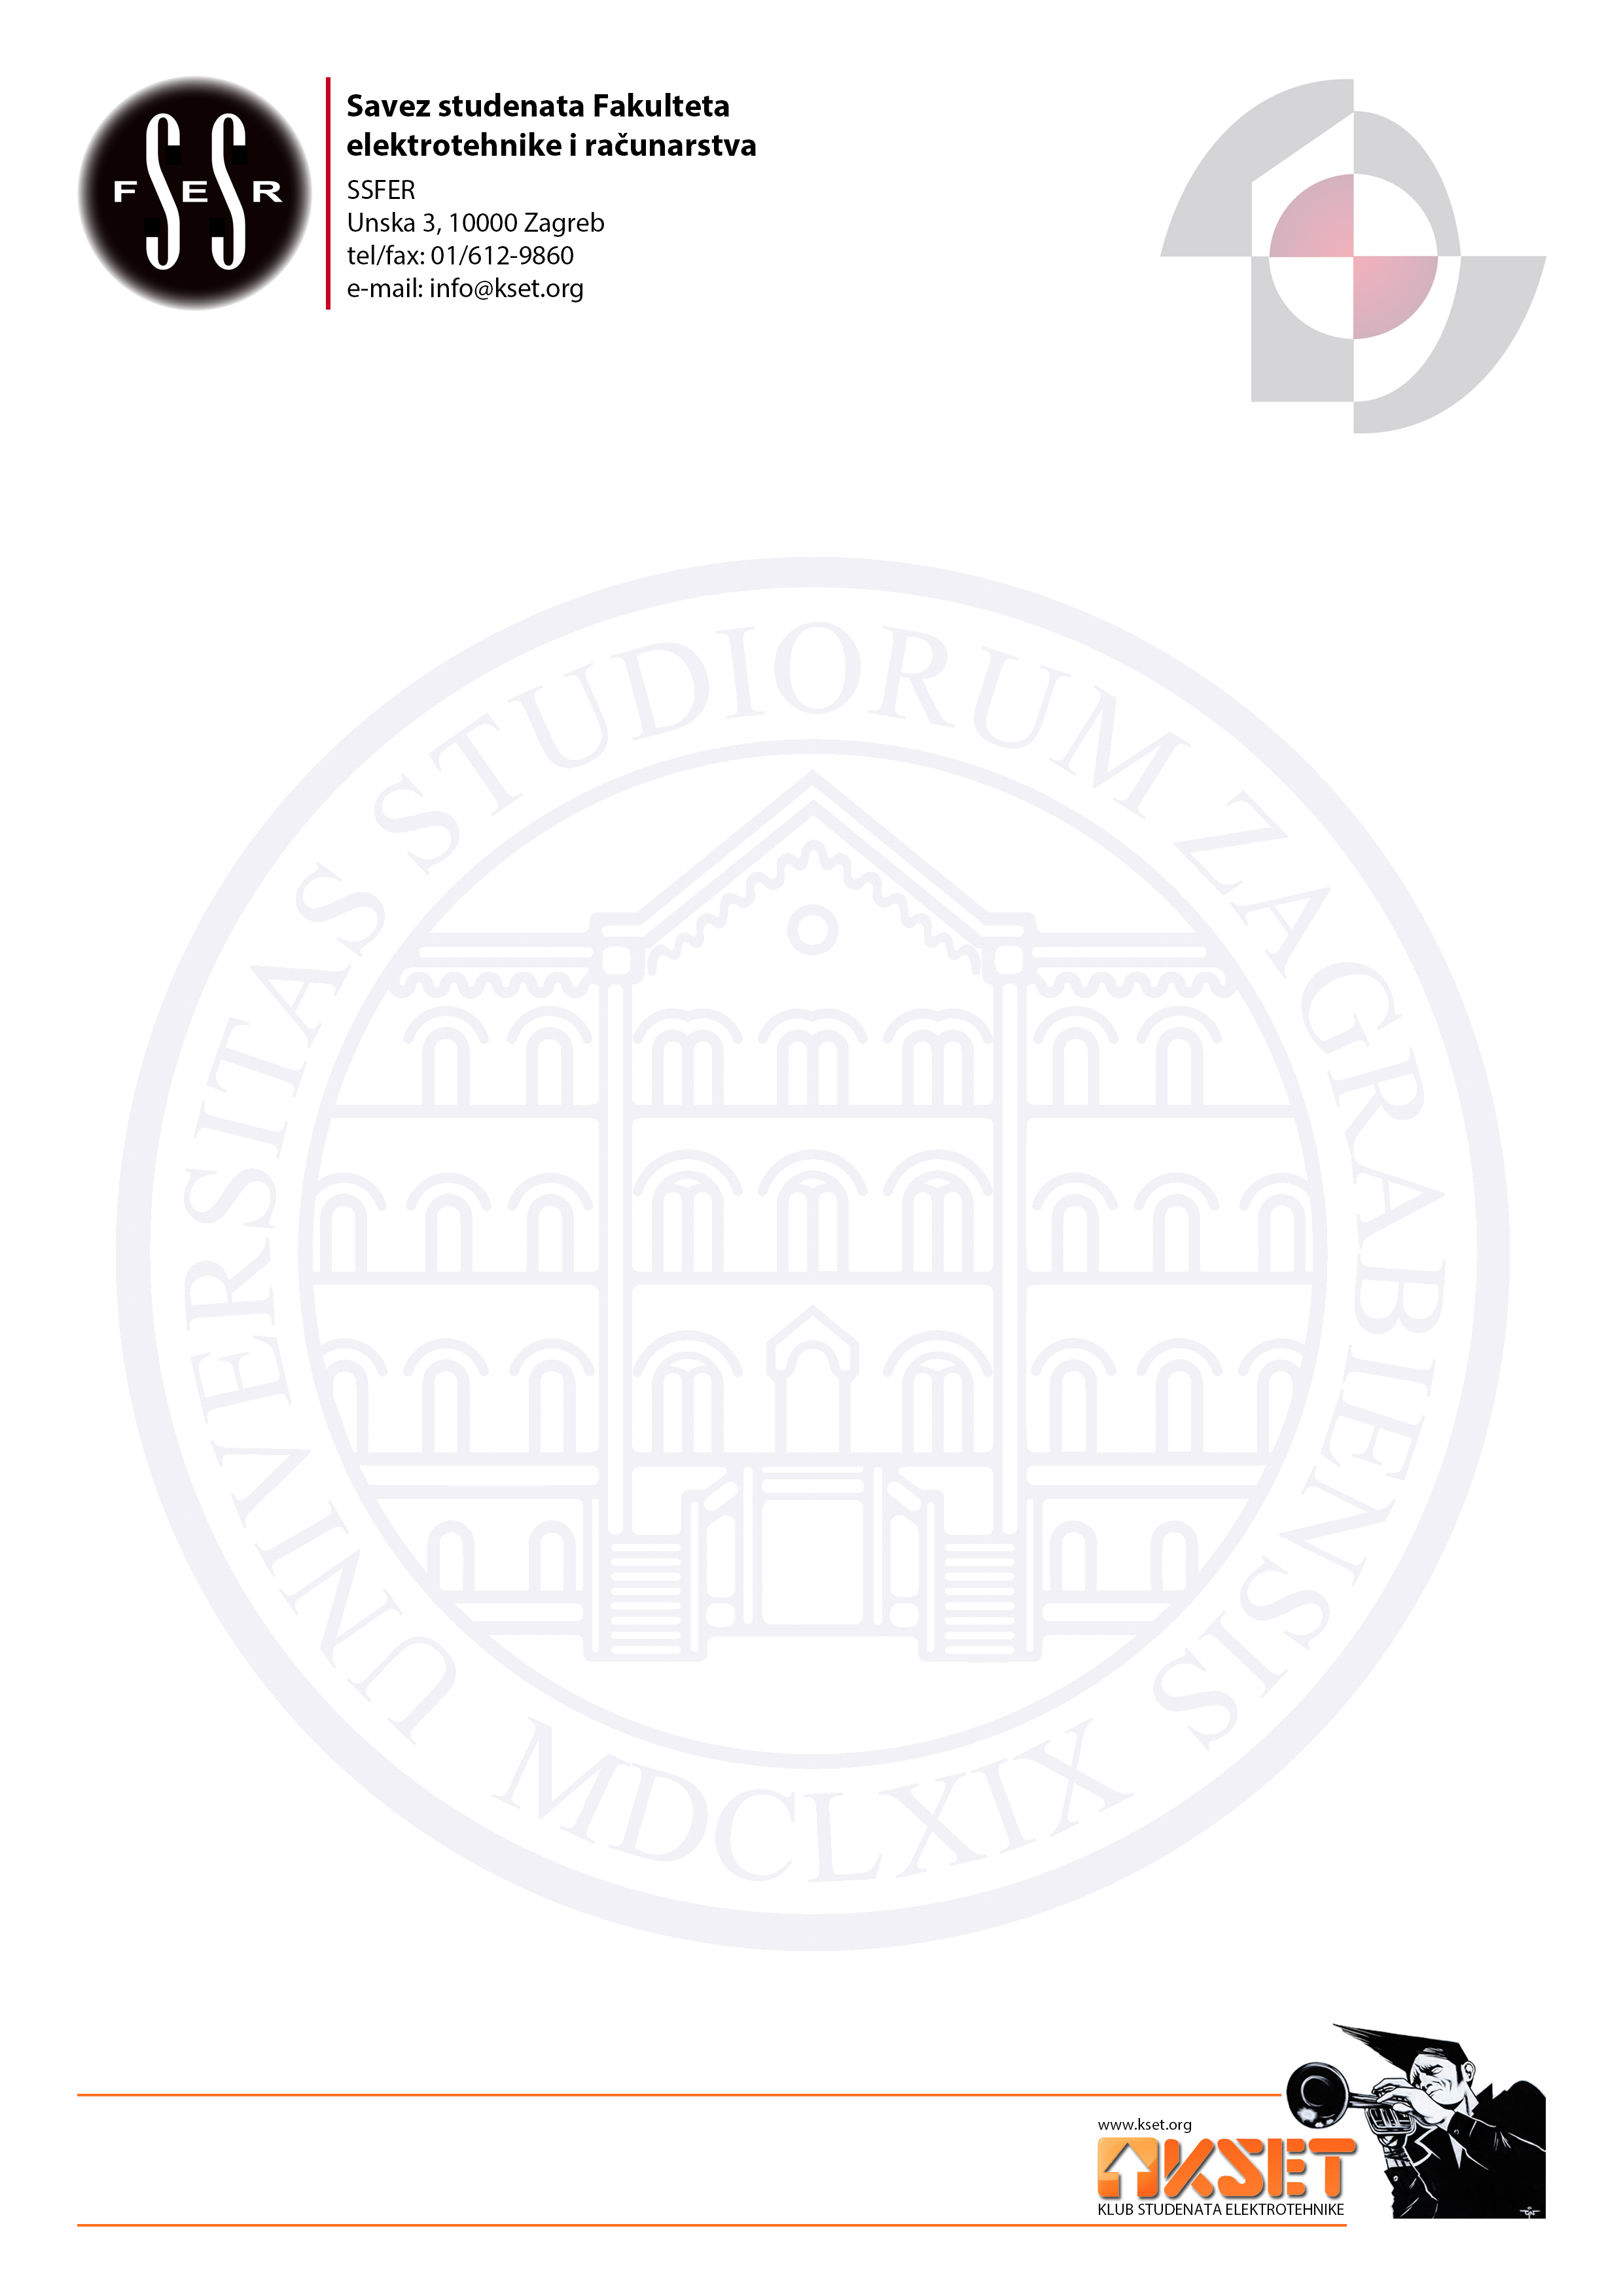
\includegraphics[width=\paperwidth,height=\paperheight]{templateBG}};

\section*{Znanstveno i tehničko djelovanje}

	\paragraph{Job Fair}je projekt čija je svrha sudjelovanje studenata tehničkih fakulteta i veleučilišta u Zagrebu te ideja da im pružimo uvid u mogućnosti zaposlenja i razvoja karijere, daljnjeg obrazovanja ili ulaska u poduzetničke vode. Događaj traje dva dana na Fakuletu elektrotehnike i računarstva gdje su izloženi štandovi tvrtki, a cijeli dan se odvijaju i predavanja u sklopu tehnološke konferencije. Putem ovog projekta želi se pružiti mogućnost tvrtkama da se približe studentima koji su njihovi potencijalni kreativni novi zaposlenici.
	
	\begin{figure}[h!]
		\centering
		\vspace{5mm}
		
\includegraphics[scale=0.35]{jobfair.png}	
	\end{figure}	
	
	\paragraph{Tech Talk}je program gdje se tijekom cijele godine održava skup radionica i prezentacija tehnološke naravi. Okuplja tvrtke i mlade poduzetnike te im pruža priliku predstaviti studentima svoje radove, zanimljive teme, izazove i rješenja s kojima se susreću u svakodnevnom poslu. Studenti se tako mogu upoznati s mogućnostima zaposlenja i razvoja karijere u Hrvatskoj i inozemstvu, a tvrtke razvijati brand i odnose među vrhunskim studentima i potencijalnim zaposlenicima.
	
	\begin{figure}[h!]
		\centering
		\vspace{5mm}
		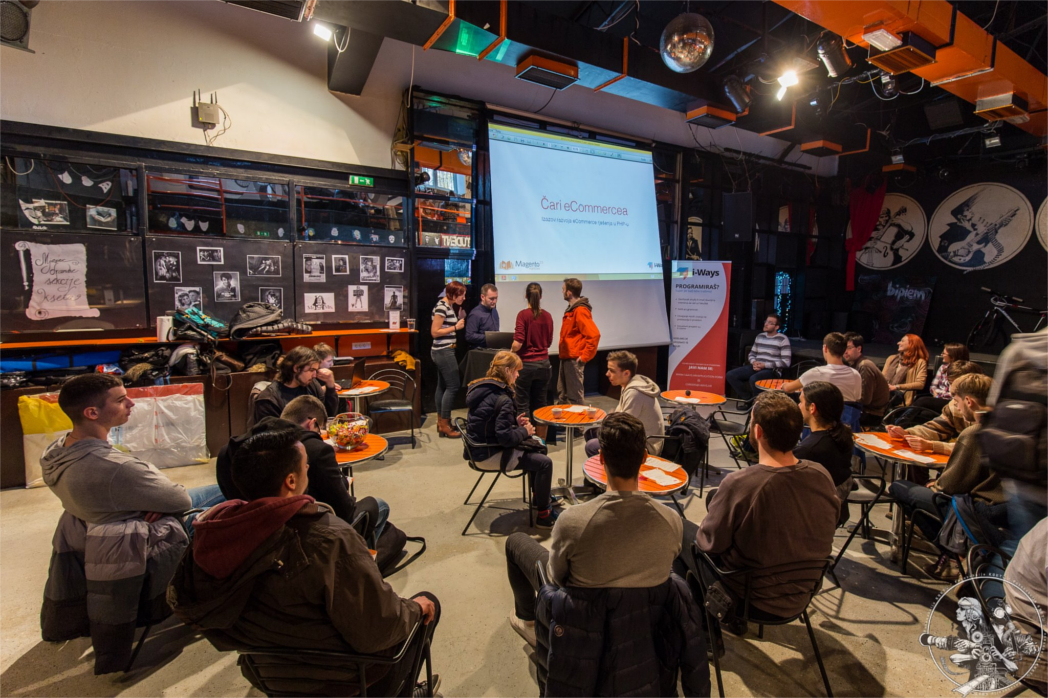
\includegraphics[scale=0.25]{techtalk.jpg}	
	\end{figure}	
	
\newpage
\tikz[remember picture,overlay] \node[opacity=1,inner sep=0pt] at (current page.center){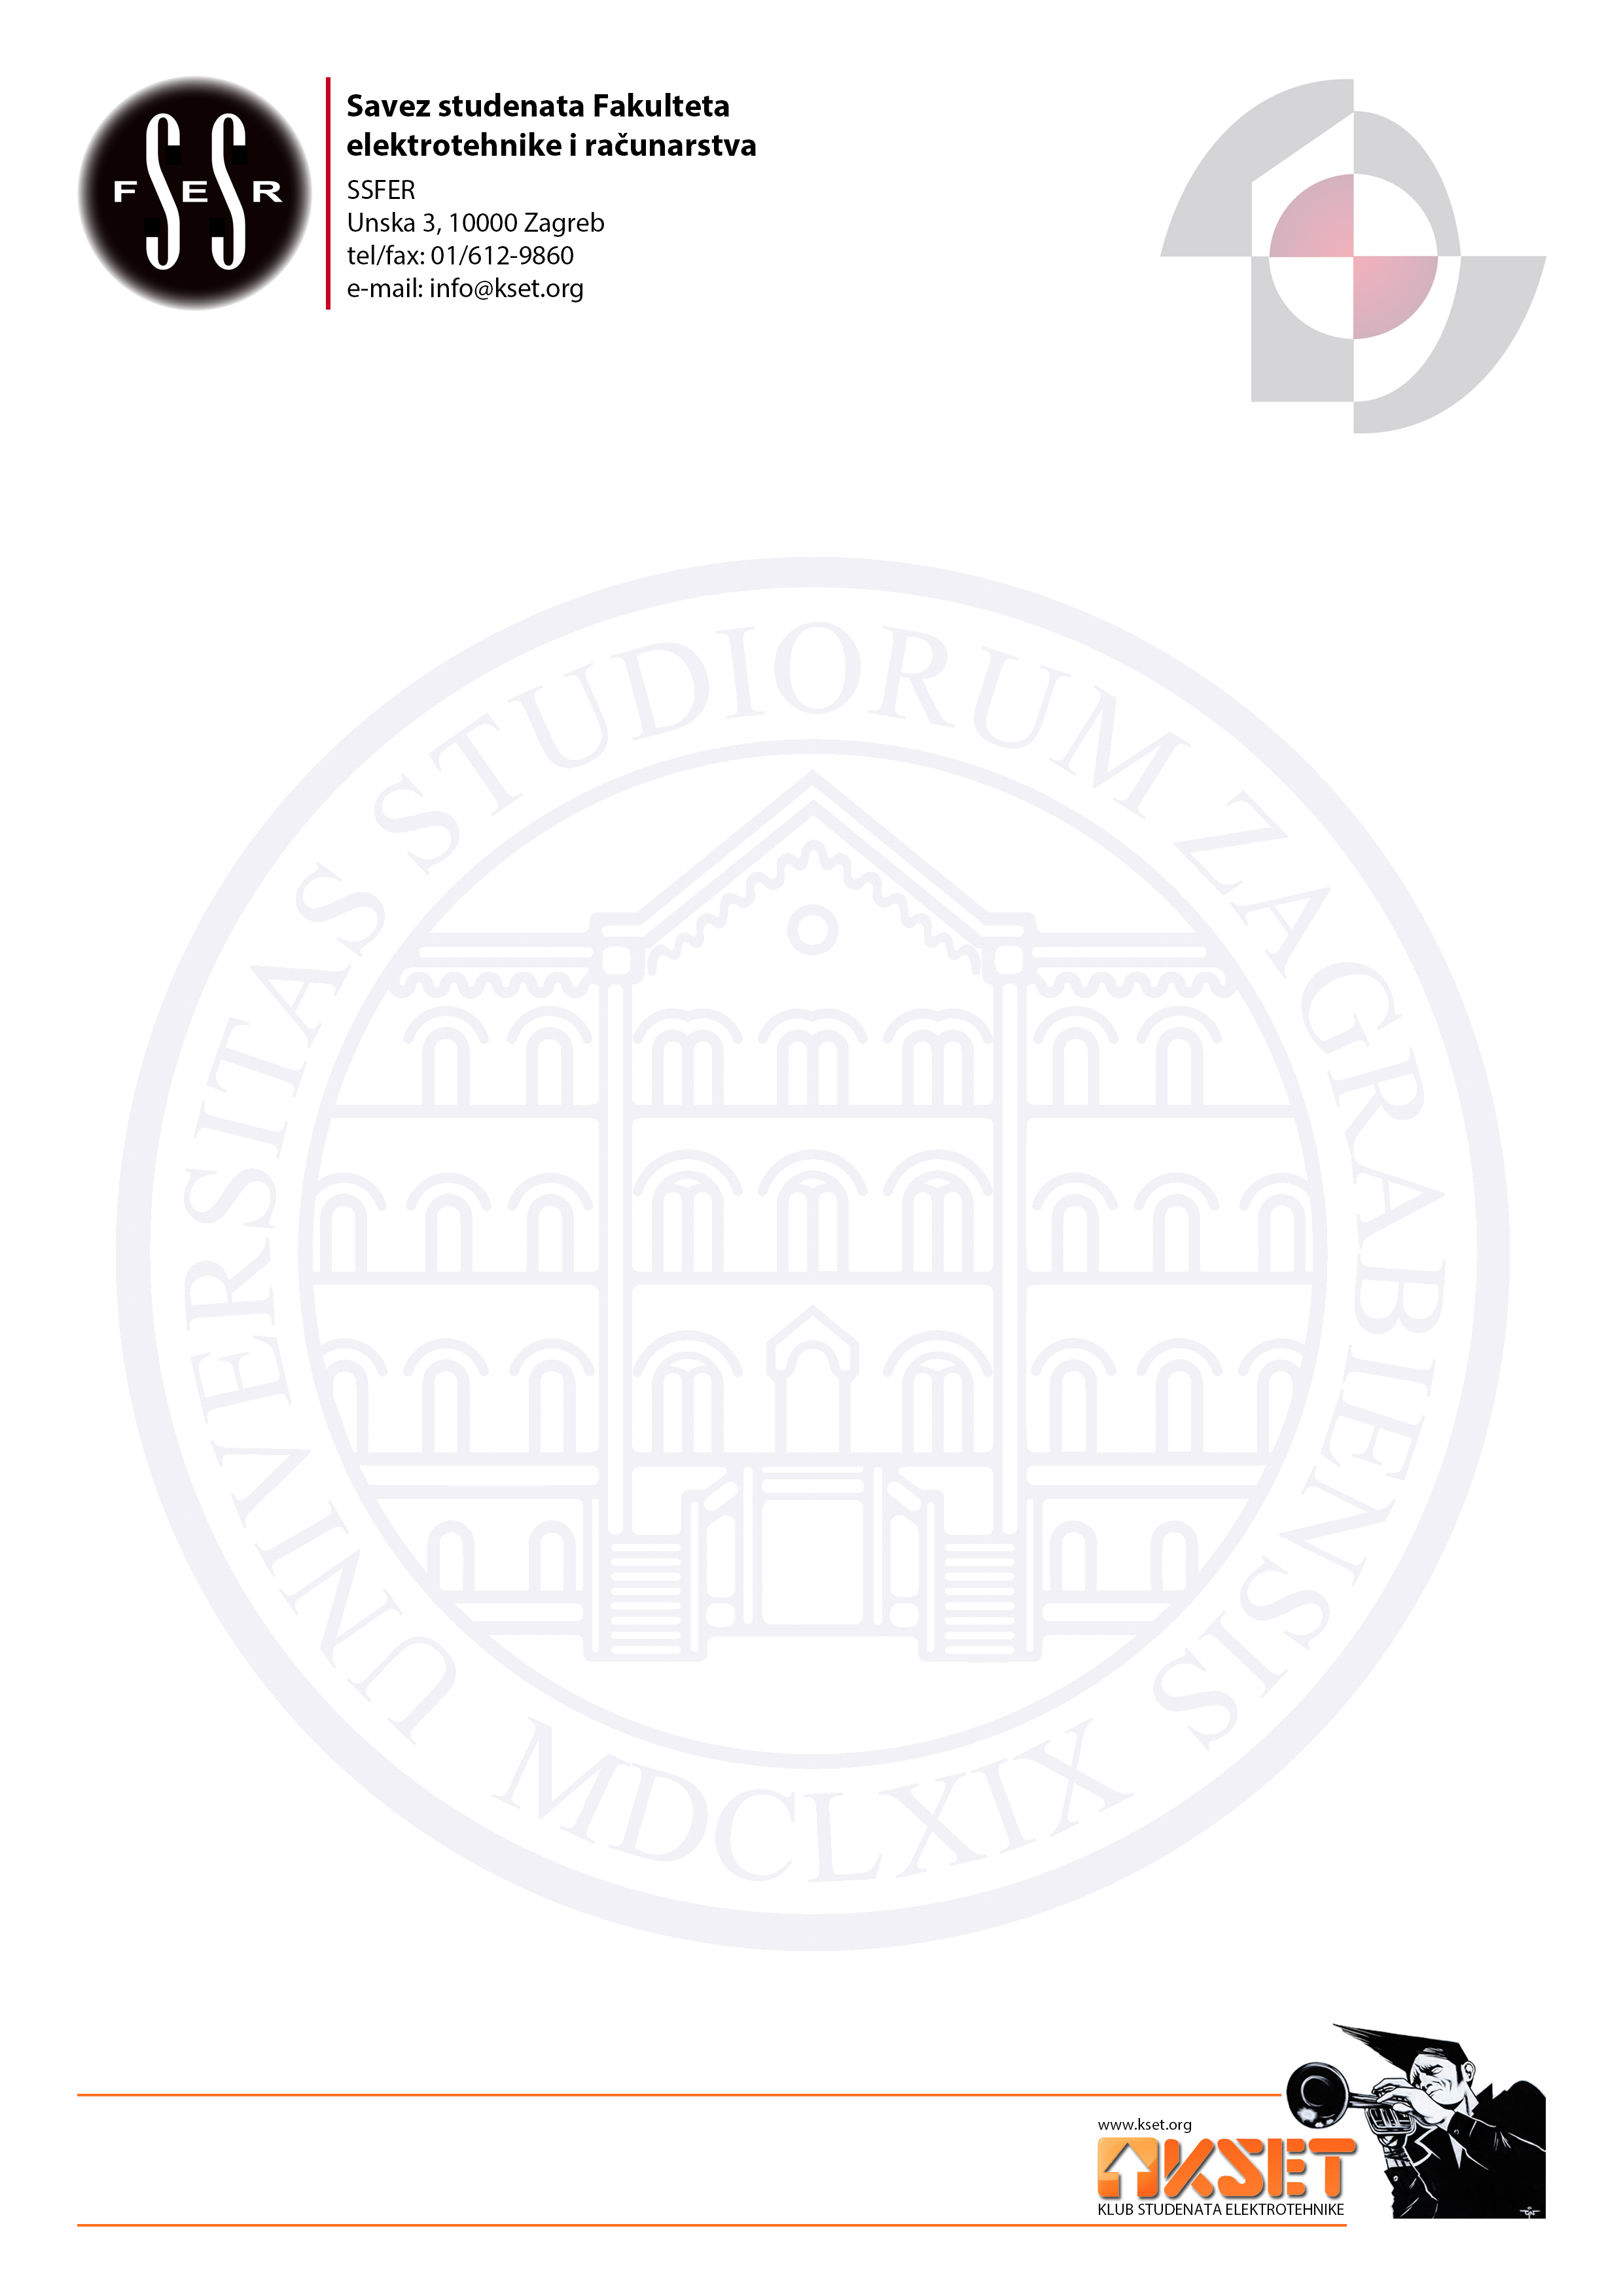
\includegraphics[width=\paperwidth,height=\paperheight]{templateBG}};	

	\paragraph{OKOSL} ili Osnove korištenja operacijskog sustava Linux  je vještina koja se održava na FER-u, a cilj joj je studentima (pogotovo onima nižih godina studija) približiti i demistificirati Linux, i pokazati da to nije sustav koji koriste samo "neckbeardovi bez života", nego sustav koji svatko može koristiti svakodnevno. Vještina je specifična po tome što ju (izuzev dijela administracije) u potpunosti organiziraju studenti - mahom stari polaznici vještine.
	 Štoviše - OKOSL je vještina zbog koje je uopće uvedena kategorija "vještine" na Fakultetu, i kao takva je prva vještina koja se održava, i to upravo na inicijativu KSET-a. Formalni je nositelj vještine profesor Stjepan Groš, koji omogućuje rezervaciju dvorana i komunicira sa Studentskom službom, ali o svemu ostalom - predavanjima, zadaćama, materijalima itd. - brinu studenti-organizatori.
	
Vještinu mogu upisati studenti svih fakulteta Sveučilišta u Zagrebu, i nije potrebno neko posebno predznanje, pa tako svake godine vještinu pohađa i nekoliko studenata Prirodoslovno-matematičkog fakulteta.
Kroz vještinu se poučavaju osnovni koncepti arhitekture UNIX sustava, poput hijerarhije datotečnog sustava i upravljanja korisnicima i dozvolama, a vještina je jako orijentirana na rad u terminalu. Rad u terminalu (i u tekstualnom korisničkom sučelju općenito) je iznimno koristan, ali ga studenti uglavnom izbjegavaju, pa je jedan od ciljeva vještine upravo ukazivanje na korisnost i jednostavnost rada s tekstualnim sučeljem, njegovo demistificiranje te uklanjanje "straha" od njegovog korištenja.

Studenti uglavnom budu vrlo zadovoljni vještinom jer prenosi skup vrlo korisnih znanja i zanimljivih koncepata, te sposobnost korištenja konkretnih i aktualnih alata, poput terminala, Git-a i regularnih izraza. Ovo se, naravno, pokazuje vrlo korisnim - kako za nastavak studija, tako i za svakodnevni rad, i većina polaznika nakon polaganja vještine ima puno dublje razumijevanje računarskih sustava.

S druge strane katedre, pak, studenti-organizatori također stječu brojne iznimno korisne vještine - predavači, primjerice, u jednom vrlo sigurnom i ugodnom okruženju stječu vještine prezentiranja, predavanja i prenošenja znanja na kolege, a oni koji sudjeluju u pripremi vježbi i zadaća postaju svjesni stvari na koje treba pripaziti pri takvom poslu, poput adekvatnog opsega i težine zadataka, te ishoda učenja.

\newpage
\tikz[remember picture,overlay] \node[opacity=1,inner sep=0pt] at (current page.center){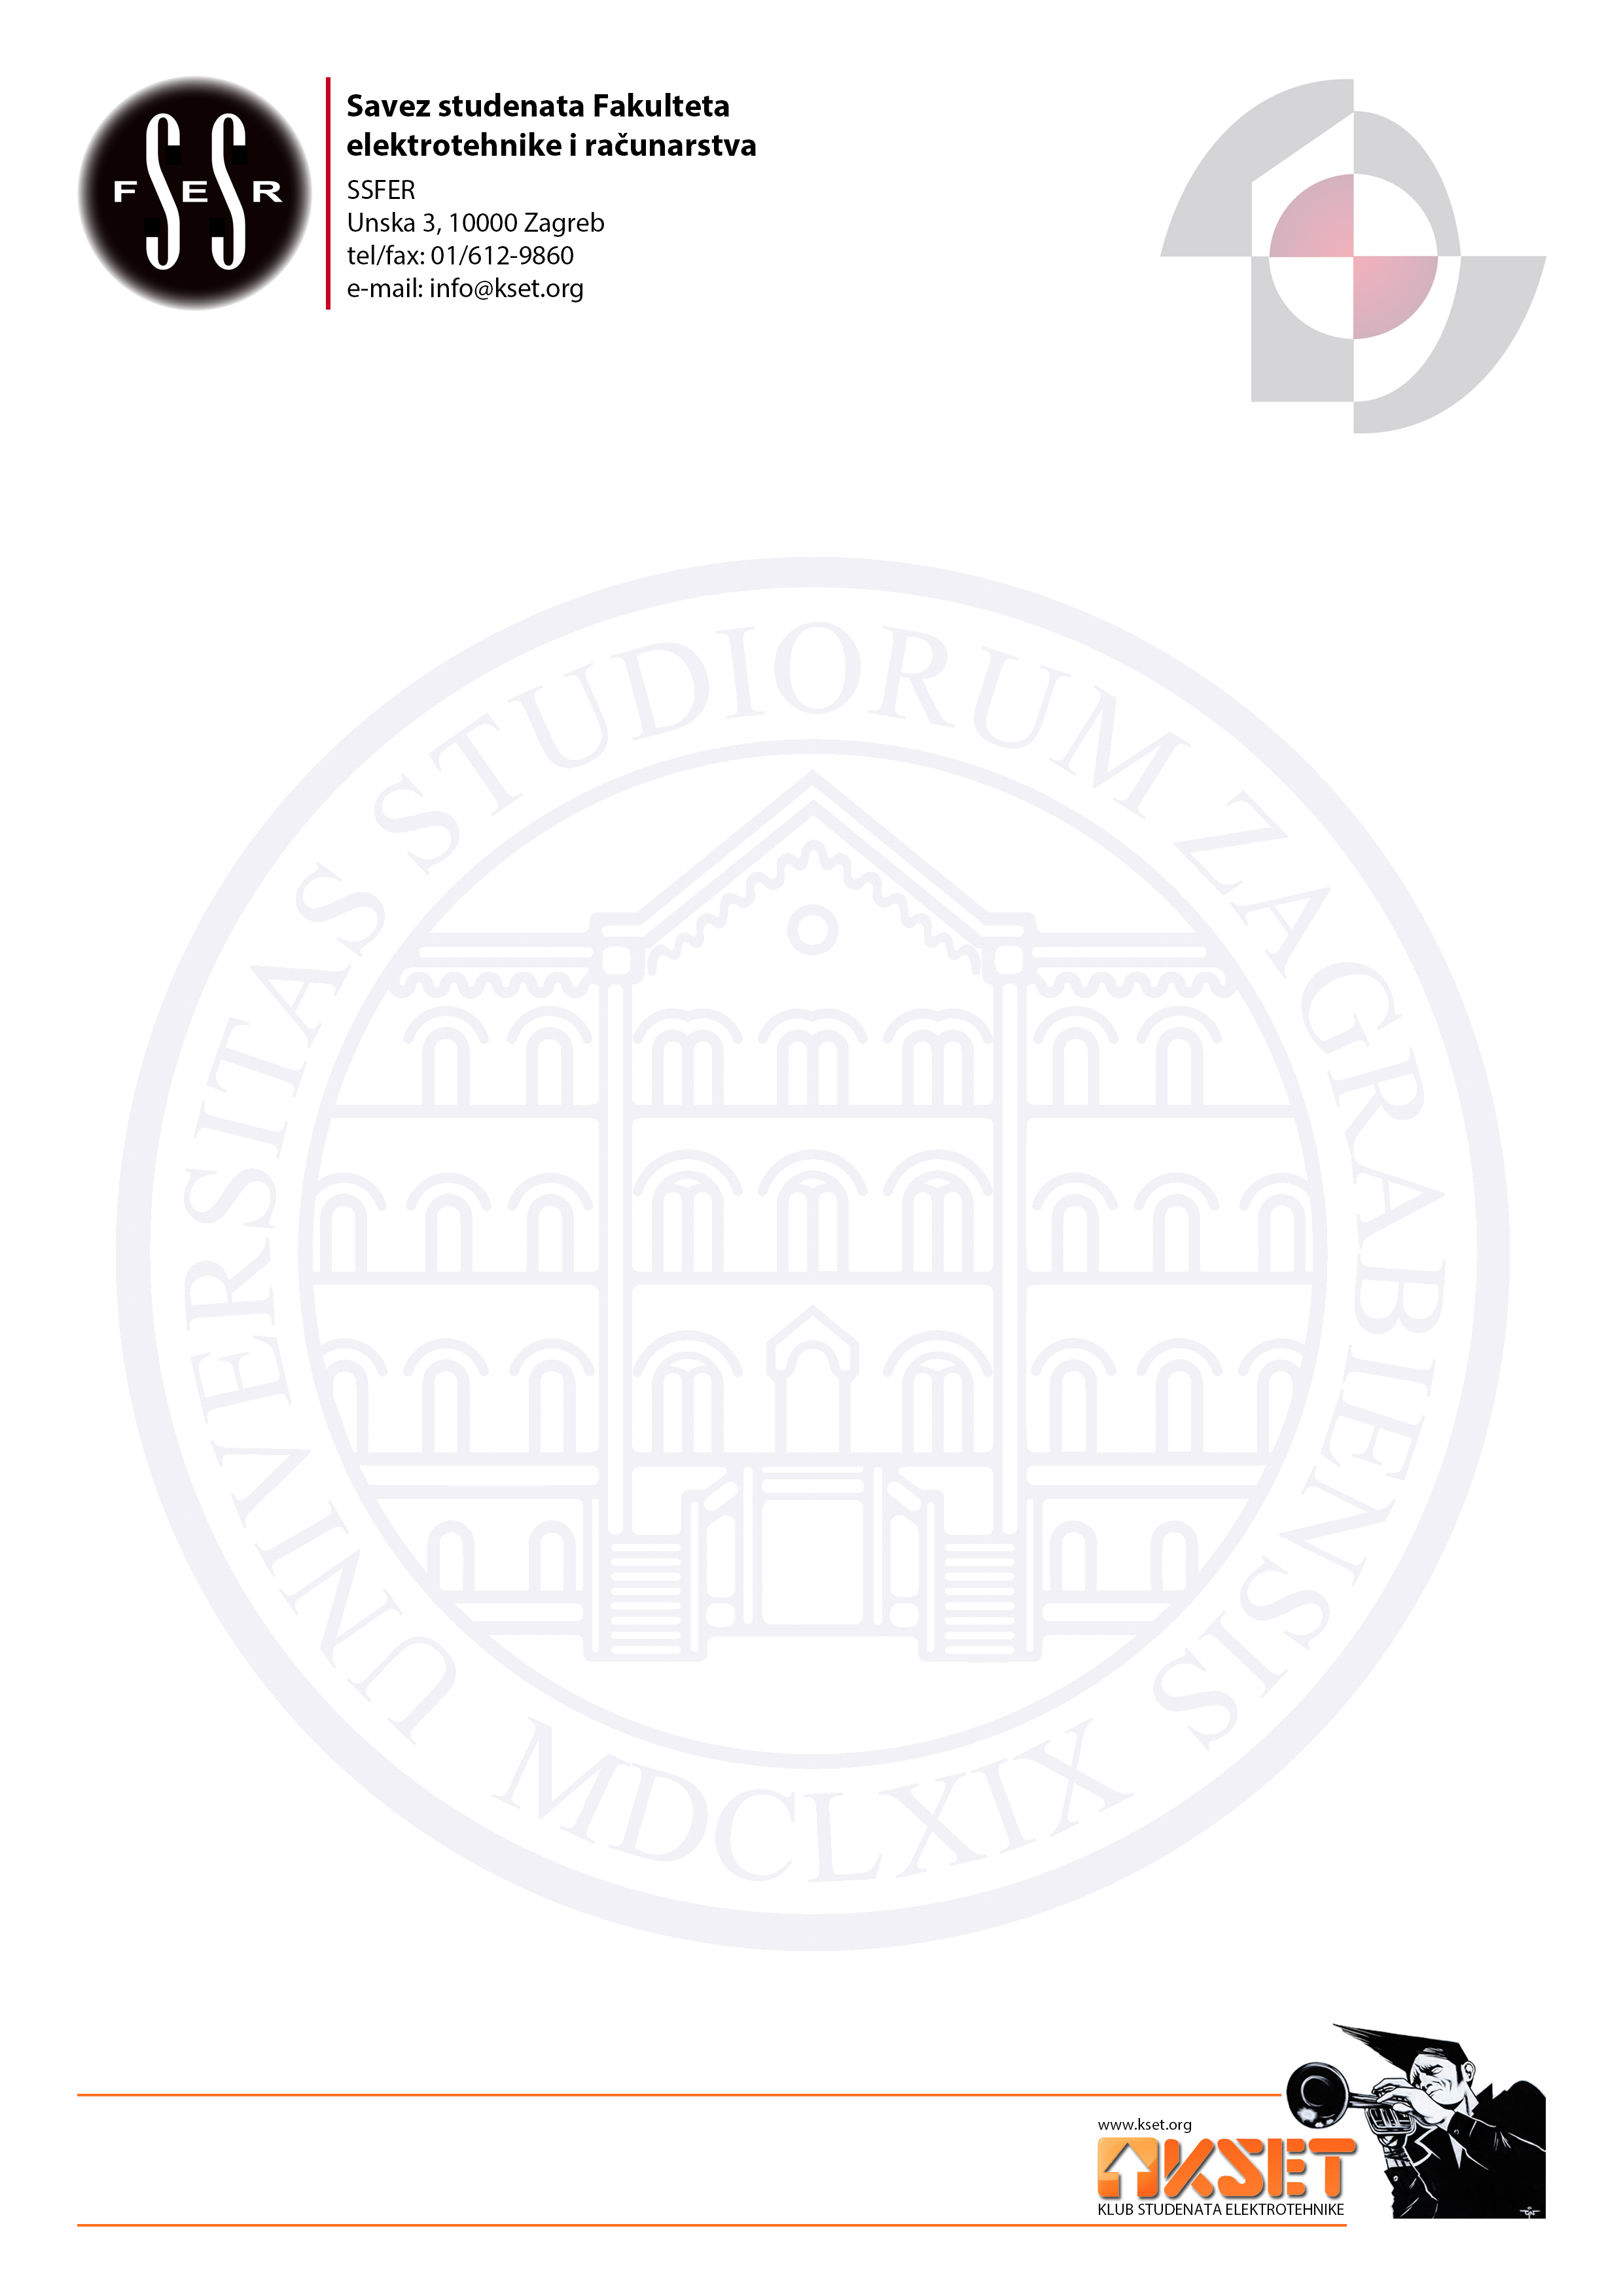
\includegraphics[width=\paperwidth,height=\paperheight]{templateBG}};	

\paragraph{NKOSL} ili Napredno korištenje operacijskog sustava Linux je vještina koja se održava na FER-u, a cilj joj je, s pretpostavkom odslušanog OKOSL-a, zaviriti u srž Linuxa i poučiti za koje je spektre zadataka Linux posebno adekvatan alat. Na NKOSL-u se znanja stečena na OKOSL-u upotrebljavaju za konkretne zadatke, poput mrežne administracije ili praćenja stanja i sigurnosti sustava - nekog serverskog okruženja, primjerice.

Vještina je posebno interesantna po tome što, osim znanja s OKOSL-a, agregira i znanja s ostalih predmeta s Fakulteta i stavlja ih u kontekst konkretne primjene i uvriježenih praksi. Na ovaj se način još više širi razumijevanje operacijskih sustava, web tehnologija, komunikacije s hardverom, te računarstva općenito. Tako studenti stječu osnovno poznavanje nekih naprednijih alata i mogućnosti dostupnih na različitim Linux distribucijama, i uvedeni su u svijet administracije računalnih sustava.

Na kraju vještine su studenti koji su položili vještinu pozvani na suradnju za održavanje ove dvije vještine. Tako se iz godine u godinu odgajaju novi predavači i demonstratori, a postoji i čvrsta sprega KSET-a i ove dvije vještine.
	

	\paragraph{Fototečaj}je tečaj za početnike i sastoji se od dva dijela: teorijskog i praktičnog. Teorijski dio  pokriva praktične osnove fotografije (osnove fotoaparata, ekspozicija, blenda, filmovi i filtri), mehaniku  fotoaparata i optički dizajn objektiva, tehnički elementi fotografije, rad s fotografskom opremom, građu i podjelu filmova te rad u tamnoj komori (razvijanje negativa i pozitiva). Detaljno se obrađuje i kompozicija u fotografiji  koja je jako bitan i u tečajevima često zanemarivan dio fotografije. Nadalje, program obrađuje digitalne fotoaparate (podjela, dijelovi, senzori  (vrste i pogreške), HDR, formate zapisa (tiff, RAW, jpeg) i načine kompresije, te analizu kvalitete fotografije pomoću histograma. Na mnoštvu primjera objašnjavaju se utjecaji tehničkih elemenata na slike te se analiziraju brojne fotografije jednostavnih i složenih kompozicija. Na kraju tečaja bit će riječ o fotografijama koje su obilježile 20. stoljeće. Tijekom tečaja polaznici će dobivati domaće zadaće preko e-learning modula FotoMoodle, preko kojega će se moći komunicirati putem foruma te na kojem će se nalaziti nastavni materijali potrebni za rad. Polaznici će dobiti i Fotoskriptu koja svojim sadržajem prati gradivo predavanja i predstavlja zaokruženu cjelinu iz osnovnih znanja o fotografiji i fotografskim procesima. U praktičnom dijelu polaznici imaju priliku u praksi primijeniti naučeno te uz iskusne fotografe na individualnoj bazi fotografiraju i u tamnoj komori razvijaju i izrađuju vlastite fotografije. Po završetku osnovnog fototečaja predviđeni su daljnji tečajevi, i to napredni tečaj rada u tamnoj komori, tečaj koncertne fotografije i tečaj studijske fotografije.
	
	\paragraph{Fotoradionica}je radionica orgnizirana od strane fotosekcije. U početku se prikazuju osnove rada fotoaparata, a zatim dijelovi fotoaparata te postavke na koje se može utjecati prilikom fotografiranja. Slijedi pojašnjenje utjecaja pojedinih postavki na izgled konačne fotografije te kratki pregled vrsta senzora unutar fotoaparata. Predavači daju nekoliko savjeta polaznicima pri kupnji fotoaparata i objektiva: na što se treba paziti i gdje su najčešće pogreške. Zatim se prelazi na praktični dio se sastoji od fotografiranja s polaznicima, uz individualnu pratnju članova Fotosekcije. Sveukupni program traje 7 sati: tri sata predavanja i četiri sata prakse na fotoaparatima. Boljim polaznicima fotoradionice nudi se da svoje fotografije izlože na web galeriji.
	
	\begin{figure}[h!]
		\centering
		\vspace{5mm}
		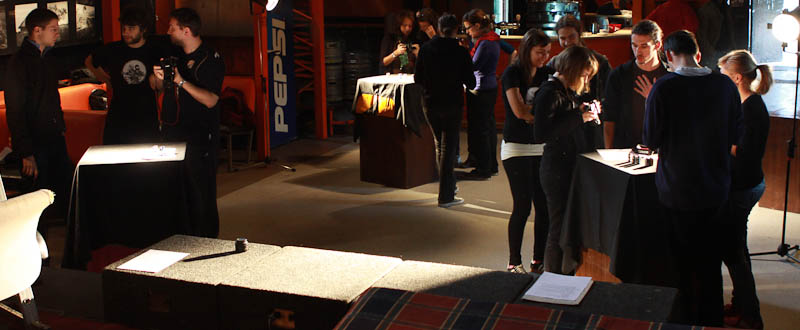
\includegraphics[scale=0.55]{fotoradionica.jpg}	
	\end{figure}
	
	\paragraph{Planinarska škola} namijenjena je za studente, asistente i profesore. Obuhvaća teorijski i terenski dio, od kojih se teorijski odvija u prostoru KSET-a, a terenski na planinama Hrvatske. Škola polaznicima pruža osnovna znanja i vještine potrbene za sigurno i odgovorno planinarenje, očuvanje okoliša te sportsku rekreaciju. Planinarsku školu vode iskusni planinari planinarske sekcije KSET-a, članovi Saveza izviđača Hrvatske, članovi Hrvatskog planinarskog društva Željezničar i članovi Planinarskog društva Sveučilišta Velebita. Oni prenose svoje bogato znanje i iskustvo koje pokriva opće znanje o planinarstvu i Hrvatskom planinarskom saveu, opasnostima u planinama, opremi, planinarskom duhu i bontonu, metodama orijentacije i navigacije na otvorenom, meteorologiji, prvoj pomoći i pristupu unesrećenom, HGSS, speleologiju, alpinizam, itd.
	
	\newpage
	\tikz[remember picture,overlay] \node[opacity=1,inner sep=0pt] at (current page.center){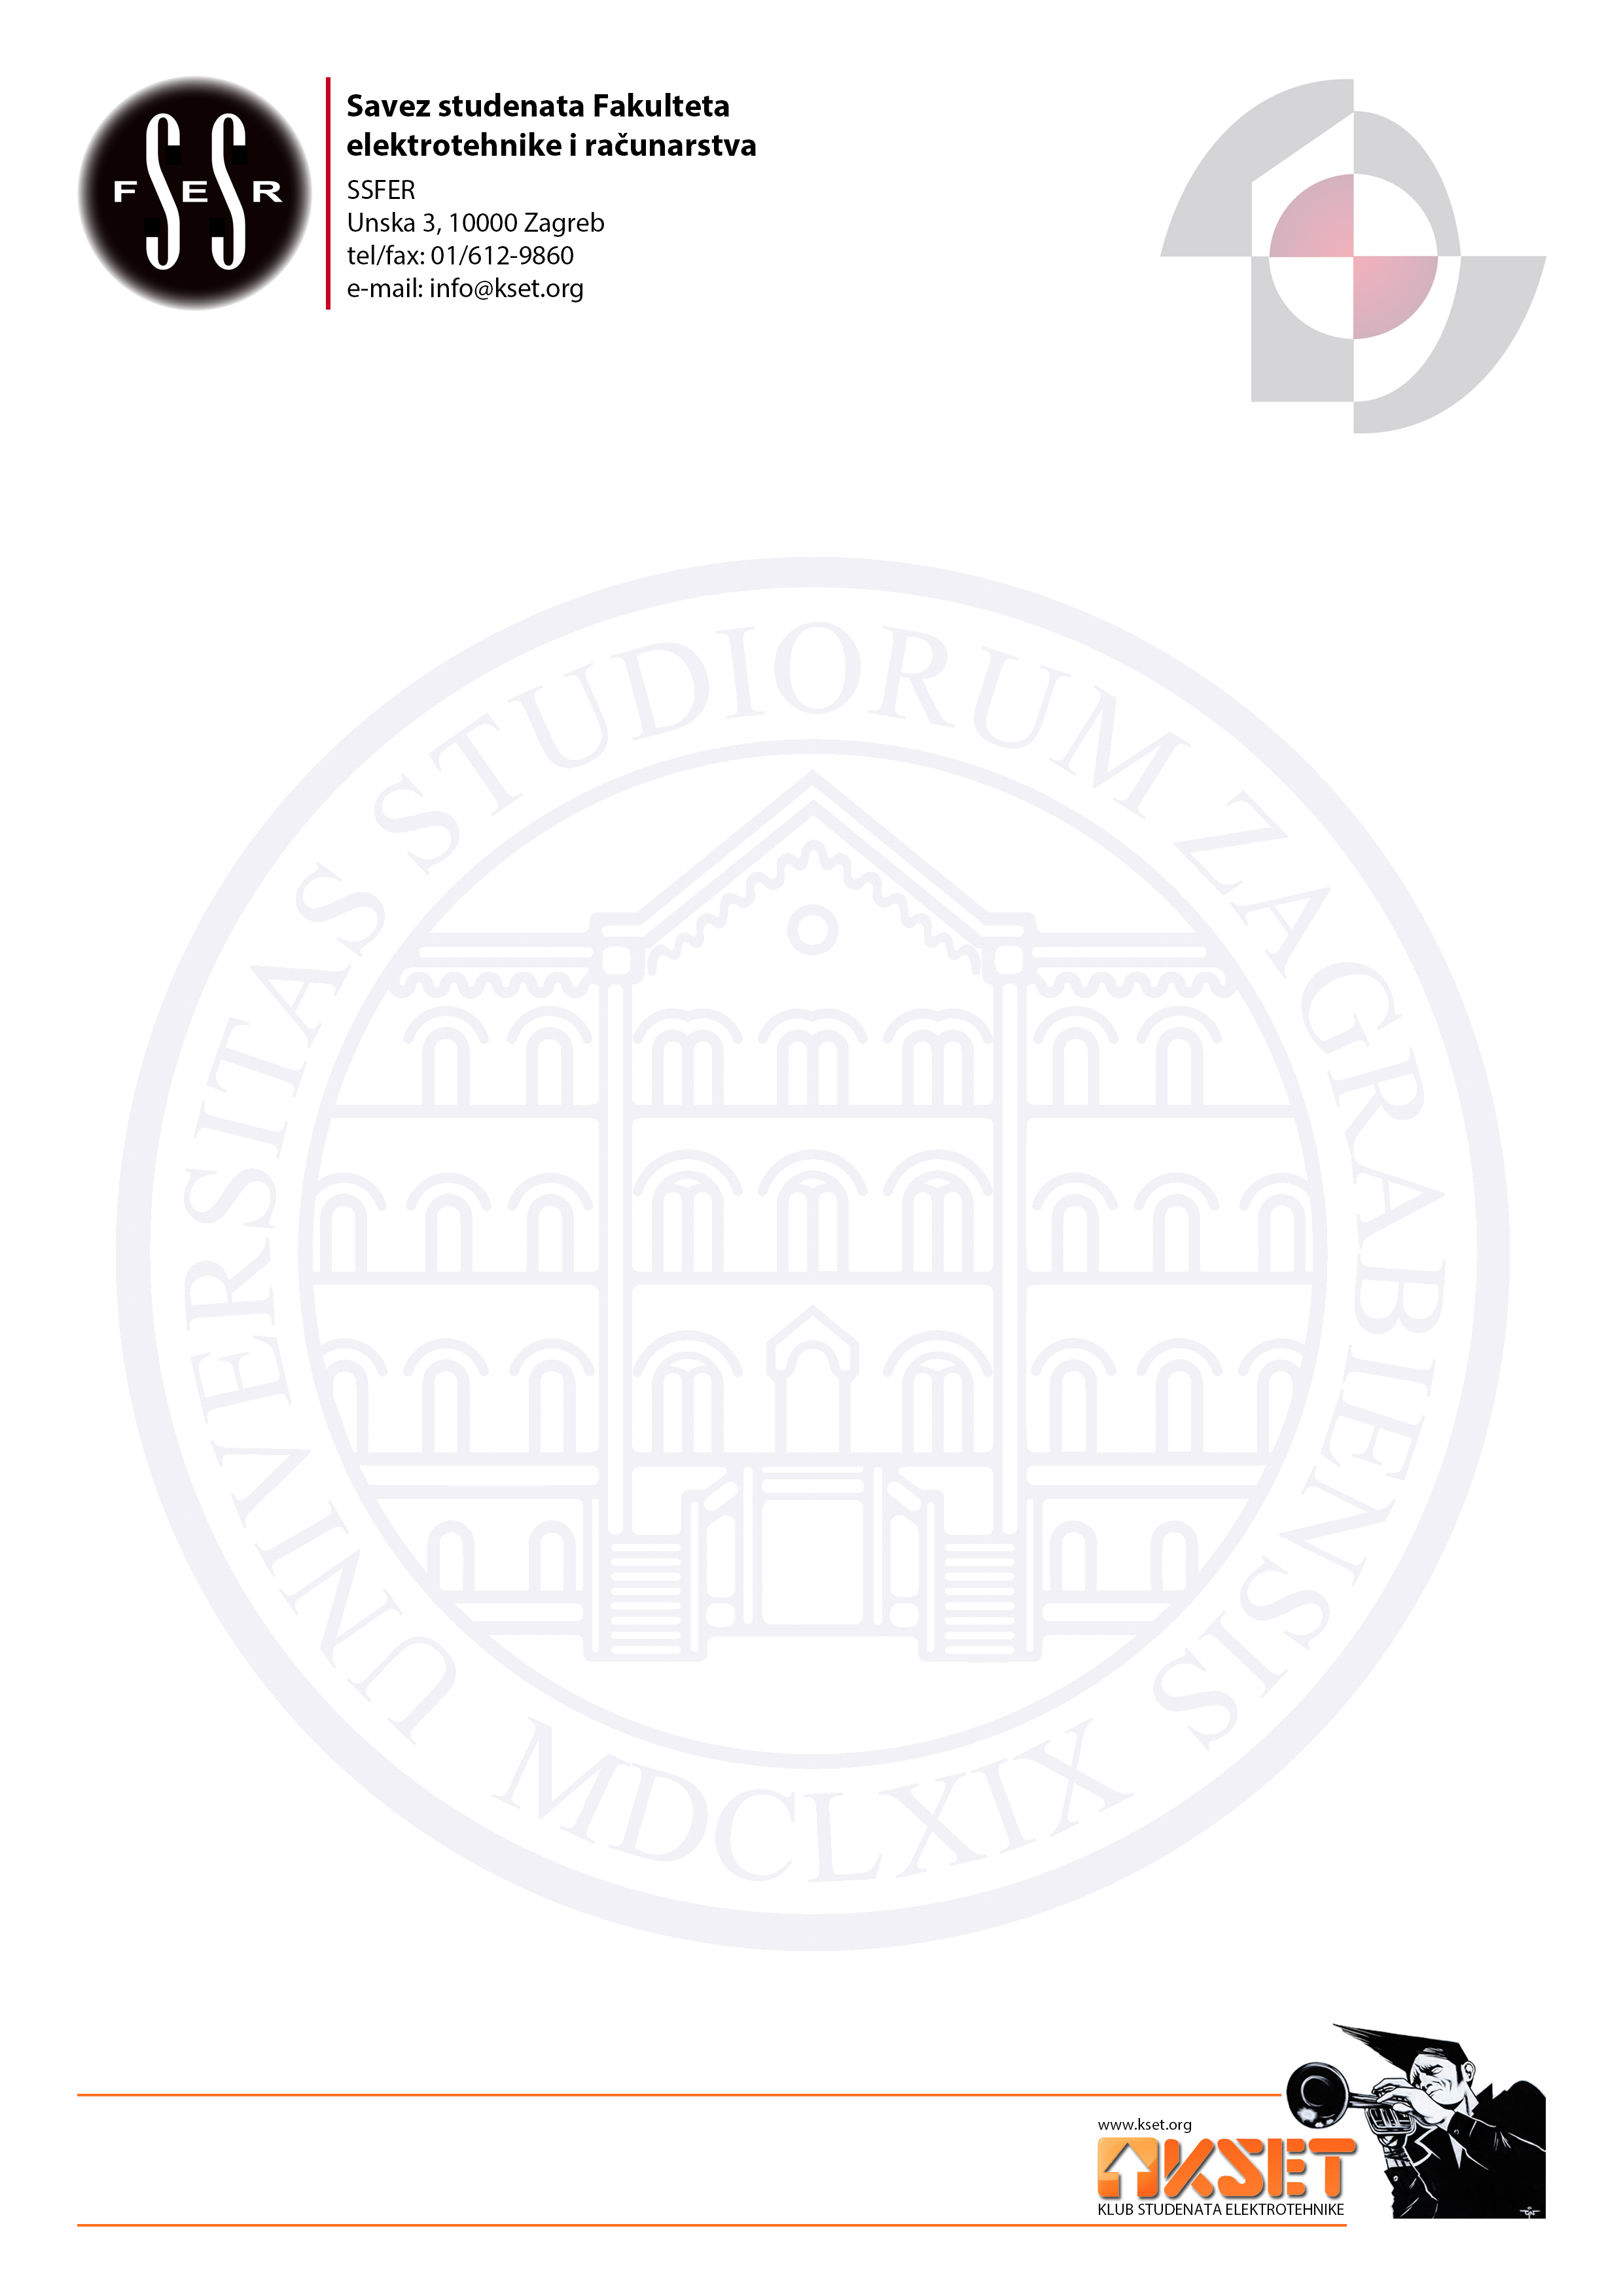
\includegraphics[width=\paperwidth,height=\paperheight]{templateBG}};
	
	\paragraph{Školice audio opreme, toniranja i obrade zvuka}je organizirana za sve audioentuzijaziste i osobe koje žele naućiti raditi u amaterskom radu obrade glazbe u neposrednoj reprodukcije. Školica sadrži predavanja o korištenju i održavanju audio opreme te u radu s osvjetljenjem izvođačkog podija. 
	
	\paragraph{Školica alata i popravaka}se sastoji od teoretskog i praktičnog dijela. Teoretski obuhvaća 3 predavanja, od kojih svako sadrži teoretsko znanje o korištenju po 2 alata. Praktični dio podrazumijeva da, nakon odslušanog teoretskog djela, svaki polaznik isproba rukovati sa svakim alatom, te stekne osnovno praktično znanje. Škola prethodi i obavezno predavanje o sigurnosti na radu, te polaznik, prije nego krene na praktični dio, ima kratak ispit iz navedenog područja.
	
		\begin{wrapfigure}{R}{0.5\textwidth}
			\vspace{-9mm}
			\begin{flushright}
				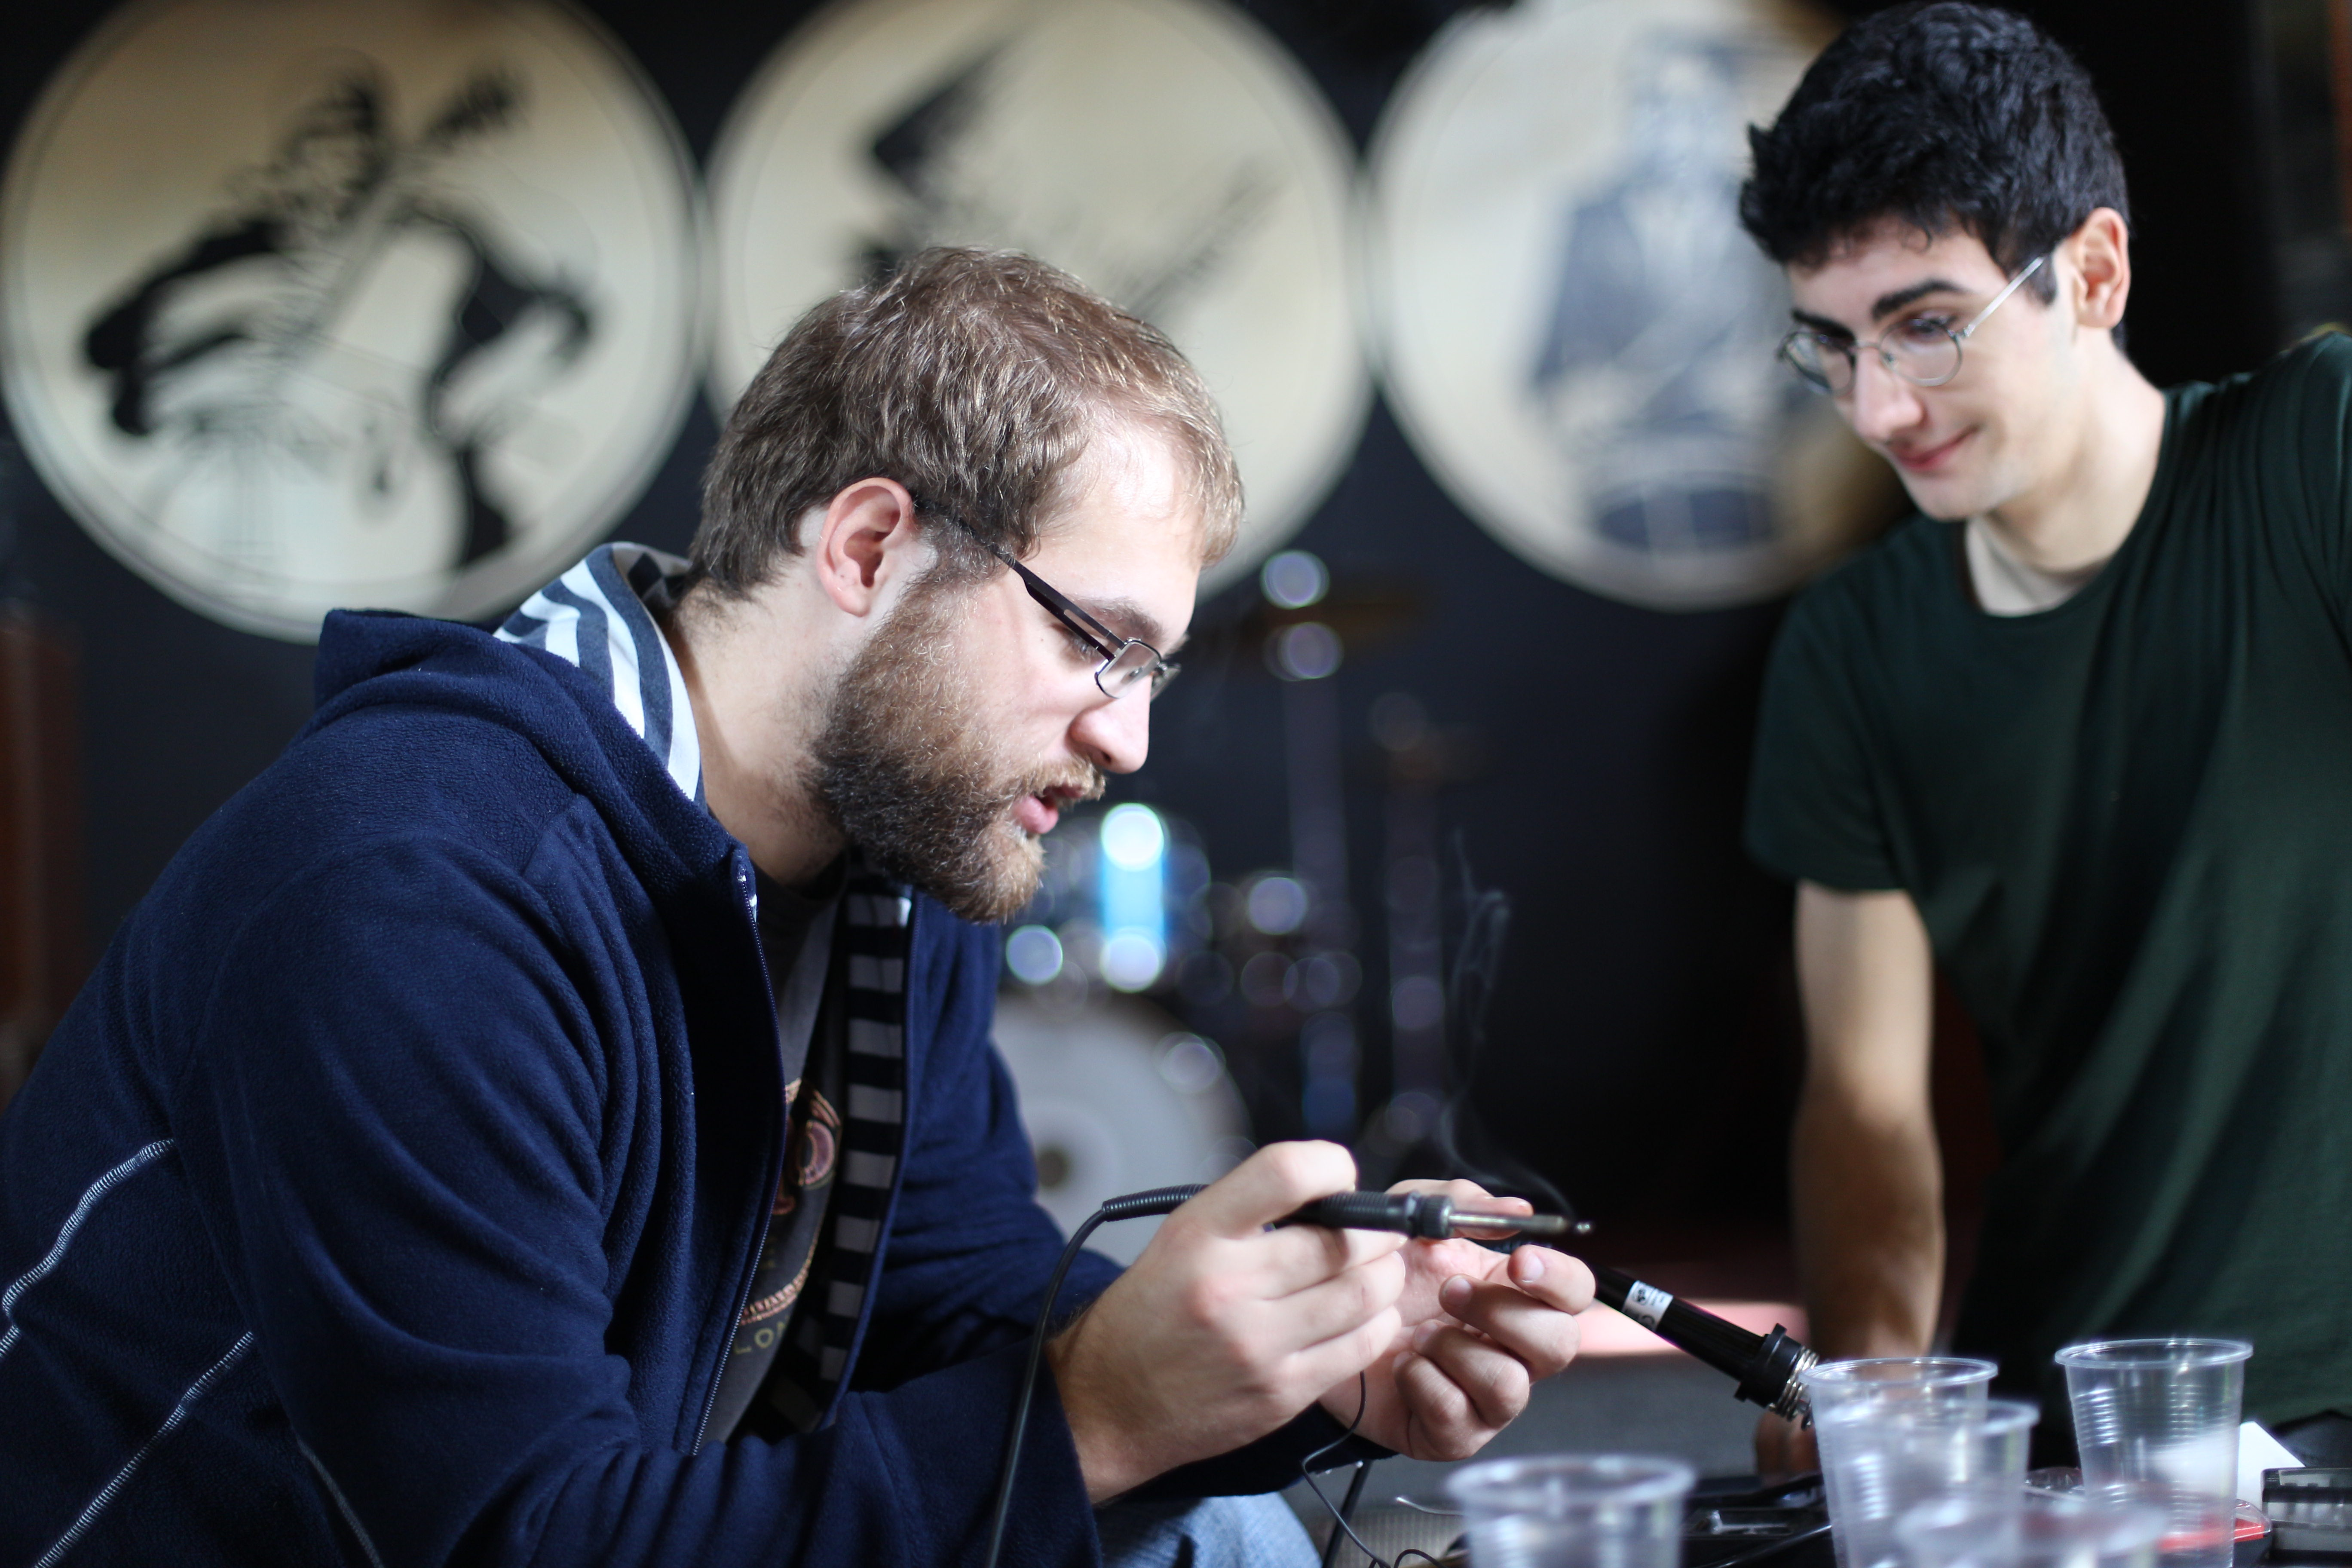
\includegraphics[width=0.5\textwidth]{elektronika.jpg}
			\end{flushright}
			\vspace{-10mm}
		\end{wrapfigure}	
	
	\paragraph{Školica praktične elektronike}organizirana je s ciljem nadopunjavanjem praktičnog znanja studenata FER-a. Laboratorijske vježbe na fakultetu često zbog nedostatka vremena i prostora nisu dovoljan izvor znanja koja se pred jednog inženjera predstavljaju u praksi. 
	Među članovima Tehničke sekcije KSET-a rodila se ideja o održavanju škole praktične elektronike koja bi upotpunila teorijsko znanje stečeno na kolegijima studija FER-a. Škola bi studentima ponudila nadopunu i produbljivanje znanja stečenih na fakultetu, a polaznici bi nakon položene škole bili u stanju samostalno ostvariti funkcionalan uređaj. Znanja koja pruža ova škola nužna su za kompletiranje obrazovanja inženjera, a fakulteti ih, uglavnom zbog manjka kapaciteta i financijskih sredstava, ne nude. Studenti bi tako, kroz program škole praktične elektronike, dobili jedinstvenu priliku steći iskustvo, primijeniti svoje znanje na stvarne projekte, i susresti se sa stvarnim problemima u projektiranju i realizaciji elektroničkih uređaja, a sve to koristeći instrumente koji im inače nisu dostupni.
	


\end{document}